\documentclass[a4paper,11pt]{jreport}

\usepackage{times}
\usepackage{amsmath}
\usepackage{amsfonts}
\usepackage{amssymb}
\usepackage{braket}
\usepackage{amsthm}
\usepackage{algorithm}
\usepackage{algpseudocode}
\usepackage[dvipdfmx]{graphicx}

\newtheorem{definition}{定義}
\newtheorem{theorem}{定理}
\newtheorem{proposition}{命題}
\renewcommand{\proofname}{証明}
\newcommand{\Continue}{\State \textbf{continue} }
\newcommand{\Break}{\State \textbf{break} }

\makeatletter
\def\thm@space@setup{\thm@preskip=3ex \thm@postskip=3ex}
\makeatletter

\setcounter{tocdepth}{3}
\setcounter{page}{-1}

\setlength{\oddsidemargin}{0.1in}
\setlength{\evensidemargin}{0.1in} 
\setlength{\topmargin}{0in}
\setlength{\textwidth}{6in} 
\setlength{\parskip}{0em}
\setlength{\topsep}{0em}

\usepackage{sie-jp}

\title{単体上における非凸関数の大域的最適化}
\author{千葉 竜介}
\degree{修士(工学)}
\advisor{久野 誉人}

\majorfield{コンピュータサイエンス}
\yearandmonth{2017年 3月}

\begin{document}
\maketitle
\thispagestyle{empty}
\newpage

\thispagestyle{empty}
\vspace*{20pt plus 1fil}
\parindent=1zw
\noindent
\begin{center}
{\bf 概要}
\vspace{5mm}
\end{center}

本論文では単体上における最適化を研究する.実行可能領域が単体の条件はとても単純であり多くの応用例を持つが,単体上の最適化問題は様々な実問題から考えられた経緯がある.目的関数の凸性は仮定しないが,非凸関数の最適化は凸関数の最適化に比べて困難であることが知られている.本論文で扱うのは,単調性を有した非凸関数である.単調性とは,変数の値を増やすと関数値もそれに伴って増大もしくは減少するような関数の性質である.このような単調関数を単体上で効率よく最適化することが本研究の目的である.単体上の単調関数最適化問題はこれまであまり研究されていないが,単体上の関数から単調関数への変換ができることを示すことで,本問題の困難さと,多くの問題の一般化になっていることを示した.単体をグリッド化して最適化する既存手法に対して,目的関数に単調性を仮定することで,単体上での下界が利用できることがわかった.その下界を利用し,単体の分割方法を定義した上で分枝限定法を実行した.さらに,この方法が多項式時間近似スキームであることを示し,実験によりアルゴリズムの有用性を確認した.

\par
\vspace{0pt plus 1fil}
\newpage

\pagenumbering{roman}
\tableofcontents
\listoffigures
\listoftables

\pagebreak
\setcounter{page}{1}
\pagenumbering{arabic}

\chapter{序論}

単体上の最適化問題はとても単純な制約条件を持ち,多くの応用例があるが,多様な実問題からこのような問題が考えられた経緯がある.単体上の最適化問題は広く研究されており,de Klerk \cite{deklerk_survey} \cite{deklerk} により,目的関数が連続である場合や二次関数である場合の,問題の困難さや最適化手法について論じられている.本研究では目的関数に凸性を仮定していないが,非凸関数の最適化は凸関数の最適化よりも困難であることが知られている.本研究で扱う問題の目的関数は,単調性を有した非凸関数である.単調性とは,変数の値を増やすとそれに伴って関数値も増加もしくは減少するような関数の性質である.目的関数と制約条件がともに単調関数であるような問題の最適化手法は Tuy \cite{tuy} \cite{tuy_survey} などにより研究されているが,本論文で扱う単調関数の単体上の最適化はこれまであまり研究されていない.本問題の解析を行い,単体における関数の下界値を利用することで単体上の関数から単調関数への変換ができることを示した.それによって,本問題が多くの問題を部分問題に持つことと,困難さがわかった.\par
提案する手法は,グリッド化した単体上の単調関数を分枝限定法で最適化するアルゴリズムである.Bomze, de Klerk \cite{bomze} は単体上の最適化問題に対して,単体をグリッド化することで多項式時間アルゴリズムを構築した.本研究では単体をグリッド化した上で,目的関数に単調性を仮定することで得た単体上の下界値を利用し,分枝限定法を実行した.分枝限定法における分枝規則には,単体を2つの単体に分割する方法を利用し,本アルゴリズムが多項式時間近似スキームであることを示した.さらに,計算実験によって本アルゴリズムの有用性を確認した.

\section{記号の定義}

\begin{table}[htb]
\begin{tabular}{ll}
表記 & 意味 \\ \hline
$ \mathbb{R} $ & 実数全体の集合 \\
$ \mathbb{R}^n $ & $ n $ 次元実数ベクトル全体の集合 \\
$ \mathbb{R}_+^n $ & すべての成分が非負である $ n $ 次元実数ベクトル全体の集合 \\
$ \mathbb{Z}_+ $ & 非負整数全体の集合 \\
$ \mathbb{Z}_+^n $ & $ n $ 次元非負整数ベクトル全体の集合 \\
$ x_i $ & $ n $ 次元ベクトル $ x $ の $ i $ 番目の成分 \\
$ x \leq y \; (x, y \in \mathbb{R}^n) $ & $ x_i \leq y_i \; (i = 1, ..., n) $
\end{tabular}
\end{table}

\section{構成}

第1章では序論を述べ,記号の定義を行った.第2章では本論文で扱う問題の定義を行い,その性質について論じる.次に第3章で関連研究の説明を行い,第4章では提案するアルゴリズムの構築方法の説明と,その計算量について論じる.第5章では数値実験の結果を紹介し,第6章で結論を述べる.

\chapter{単体上の単調関数最適化問題}

本章では,本論文で扱う問題の説明をする.以下のような単調関数 $ f $ の最小化問題を考える.\par

$$
\left| \;
\begin{aligned}
& 最小化 && f(x) &&&&& \\
& 条件 && \sum_{i=1}^n x_i = 1 \notag \\
& && x_i \geq 0, i = 1, ..., n \notag
\end{aligned}
\right.
$$

変数 $ x \in \mathbb{R}^n $ の各成分の和が $ 1 $ であることと非負であることが制約条件とされている.このような条件を満たす $ x $ の集合は単体と呼ばれており,de Klerk \cite{deklerk_survey} などにより様々な研究がなされている.まずは単調関数と単体を定義し,それらの性質について論ずる.\par

\section{単調関数の定義とその性質}

単調関数の定義を行う.単調関数とは,単調増加関数または単調減少関数のことであり,入力の増加に対して関数値もそれに伴って増加または減少する関数である.さらに,そのような性質を単調性と呼ぶ.単調増加関数を以下のように定義する.

\begin{definition}
$ I \subseteq \mathbb{R}^n $ 上の関数 $ f : I \to \mathbb{R} $ は任意の $ x, x' \in I $ に対して以下が成り立つ場合に単調増加関数であるという.
$$ x \leq x' \Rightarrow f(x) \leq f(x') $$
\end{definition}

一方,単調減少関数は以下のように定義できる.

\begin{definition}
$ I \subseteq \mathbb{R}^n $ 上の関数 $ f : I \to \mathbb{R} $ は任意の $ x, x' \in I $ に対して以下が成り立つ場合に単調減少関数であるという.
$$ x \leq x' \Rightarrow f(x) \geq f(x') $$
\end{definition}

ここで $ I $ は $ n $ 次元実数空間全体や区間,離散的な空間などが考えられる.また,ここで定義した単調増加関数は広義単調増加関数や単調非減少関数と呼ばれることがあるが,本論文では狭義単調増加関数を扱わないため,単に単調増加関数ということにする.単調減少関数についても同様である.

\begin{proposition} \label{prop:keeping_monotonicity}
$ f : I \to \mathbb{R} $ が単調増加関数であることと,$ -f $ が単調減少関数であることは同値である.

\begin{proof}
$ f $ は単調増加関数であるから,任意の $ x, x' \in I $ について以下が成り立つ.
\begin{align*}
& x \leq x' \Rightarrow f(x) \leq f(x') \\
\Longleftrightarrow \hspace{8pt} & x \leq x' \Rightarrow -f(x) \geq -f(x')
\end{align*}
これは $ -f $ が単調減少関数であることを示し,$ f $ が単調増加関数であることと,$ -f $ が単調減少関数であることが同値であることが証明された.
\end{proof}

\end{proposition}

命題 \ref{prop:keeping_monotonicity} より,関数値を $ -1 $ 倍する操作によって単調増加と単調減少が相互に変換され,単調性は失われないことがわかる.さらに,最適化問題において,ある関数 $ f $ を最大化することは $ -f $ を最小化することと同じであるため,関数値を $ -1 $ 倍することで最大化問題を最小化問題に変換することができる.ここからは単調増加関数の最小化問題についてしか論じないが,この通り関数値を $ -1 $ 倍することで最大化問題は最小化問題に変換することができ,その操作を行っても単調性は保存されることから,一般性は失わない.\par

\section{単体の定義とその性質}

本節では単体の定義を行う.

\begin{definition}
各成分の和が $ 1 $ である以下のようなベクトルの集合 $ \Delta_n $ を単位単体という.
$$ \Delta_n \triangleq \Set{ x \in \mathbb{R}^n_{+} | \sum_{i=1}^{n} x_i = 1 } $$
\end{definition}

単体とは,成分の和が定数になっているベクトルの集合であり,単位単体を一般化した単体を以下のように定義する.

\begin{definition}
非負実数 $ c \in \mathbb{R}_+ $ を用い,単位単体を $ c $ 倍したものを単体という.
$$ c \Delta_n \triangleq \Set{ x \in \mathbb{R}^n_{+} | \sum_{i=1}^{n} x_i = c } $$
\end{definition}

$ n $ について具体的に考えてみると,$ n=2 $ の単体は線分,$ n=3 $ の単体は正三角形,$ n=4 $ の単体は正四面体となることがわかる.このように,単体は $ n $ に対して一次元少ない $ n - 1 $ 次元空間上に存在することがわかり,一般に $ n = k $ の単体は $ k - 1 $ 次元単体と呼ばれる.よって,1次元単体は線分,2次元単体は正三角形,3次元単体は正四面体である.\par

\section{単体上の単調関数の性質}

単体の定義から以下が言える.

\begin{proposition} \label{prop:inequality_on_simplex}
単体上の任意の異なる点 $ x, y \in c \Delta_n $ について $ x \leq y $ が成り立つことはない.

\begin{proof}
背理法で示す.$ x \leq y $ となるような異なる点 $ x, y $ が $ c \Delta_n $ 中に存在すると仮定する.\\
$ x \leq y $ であるから,それぞれの成分について以下が成り立つ.
$$ x_i \leq y_i \;, i = 1, ..., n $$
さらに,$ x , y $ は異なる点であったから $ x \neq y $ であり,狭義な不等号 $ x_i < y_i $ が成り立つような $ i $ が存在する.よって $ x, y $ の成分の和に以下のような狭義の不等号が成り立つ.
$$ \sum_{i=1}^n x_i < \sum_{i=1}^n y_i $$
これは $ x, y \in c \Delta_n $ つまり,$ \sum_{i=1}^n x_i = \sum_{i=1}^n y_i = c $ に矛盾する.\\
よって,$ x \leq y $ が成り立つような単体上の異なる点 $ x, y $ は存在しない.
\end{proof}

\end{proposition}

この命題から,単調増加関数の定義である $ x \leq y \Rightarrow f(x) \leq f(y) $ を利用できる点が単体上には存在しないことがわかり,単体上だけを見ると単調関数は特に性質のない関数であるように見える.このことから,単体上の単調関数の最適化問題の困難さがうかがえる.

\section{単体上の関数から単調関数への変換}

単体 $ c \Delta_n $ 上の関数を $ \mathbb{R}_+^n $ 上の単調増加関数に変換できることを示す.まずはある領域における関数の下界値と上界値を定義する.

\begin{definition}
領域 $ A \subseteq \mathbb{R}^n $ における関数 $ f $ の下界値を $ \underline{f}_A $ としたとき,以下が成り立つ.
$$ \forall x \in A, \; f(x) \geq \underline{f}_A $$
\end{definition}

\begin{definition}
領域 $ A \subseteq \mathbb{R}^n $ における関数 $ f $ の上界値を $ \overline{f}_A $ としたとき,以下が成り立つ.
$$ \forall x \in A, \; f(x) \leq \overline{f}_A $$
\end{definition}

ここで一般に,下限値以下の値は全て下界値となるため,下界値は複数存在するが,ここでは以下を満たすもののみを $ \underline{f} $ として扱う
$$ \forall A, B \subseteq \mathbb{R}^n, \; A \subseteq B \Rightarrow \underline{f}_A \geq \underline{f}_B $$
同様に上界値についても,以下を満たすもののみを $ \overline{f} $ として扱う
$$ \forall A, B \subseteq \mathbb{R}^n, \; A \subseteq B \Rightarrow \overline{f}_A \leq \overline{f}_B $$
この設定の妥当性について考えてみると,一般に,関数値の下限について
$$ \forall A, B \subseteq \mathbb{R}^n, \; A \subseteq B \Rightarrow \inf_{x \in A}f(x) \geq \inf_{x \in B}f(x) $$
が成り立つことと,上限について
$$ \forall A, B \subseteq \mathbb{R}^n, \; A \subseteq B \Rightarrow \sup_{x \in A}f(x) \leq \sup_{x \in B}f(x) $$
が成り立つことを考えると自然であることがわかる.\par
以上のような下界値と上界値を利用し,単体を含むような領域 $ D \supseteq c \Delta_n $ で定義されている関数を $ f : D \to \mathbb{R} $ としたとき,$ \hat{f} : \mathbb{R}_+^n \to \mathbb{R} $ を以下のように定義する.

\begin{align*}
\hat{f}(x) =
\begin{cases}
\underline{f}_{A_x}, \; A_x = \Set{x' \in c \Delta_n | x' \geq x } & ( \: \mbox{If } \sum_{i=1}^{n}x_i \leq c \: ) \\
\overline{f}_{c \Delta_n} & (\mbox{ Otherwise })
\end{cases}
\end{align*}

ここで,$ \sum_{i=1}^{n}x_i \leq c $ である条件は,原点から見たときに $ x $ が単体の内側にある条件であり,一方 $ \sum_{i=1}^{n}x_i > c $ である条件は $ x $ が単体の向こう側にあることである.\par
ある点 $ x $ を選んだときの,$ A_x $ を図 \ref{fig:a_on_simplex} に図示した.薄い青色の領域が元の単体 $ c \Delta_n $,赤い点が $ x $,濃い青色の領域が $ A_x $ を表している.$ A_x $ が単体の部分領域となっており,$ A_x $ の要素はすべて $ x $ 以上であることがわかる.\par

\begin{figure}
\begin{center}
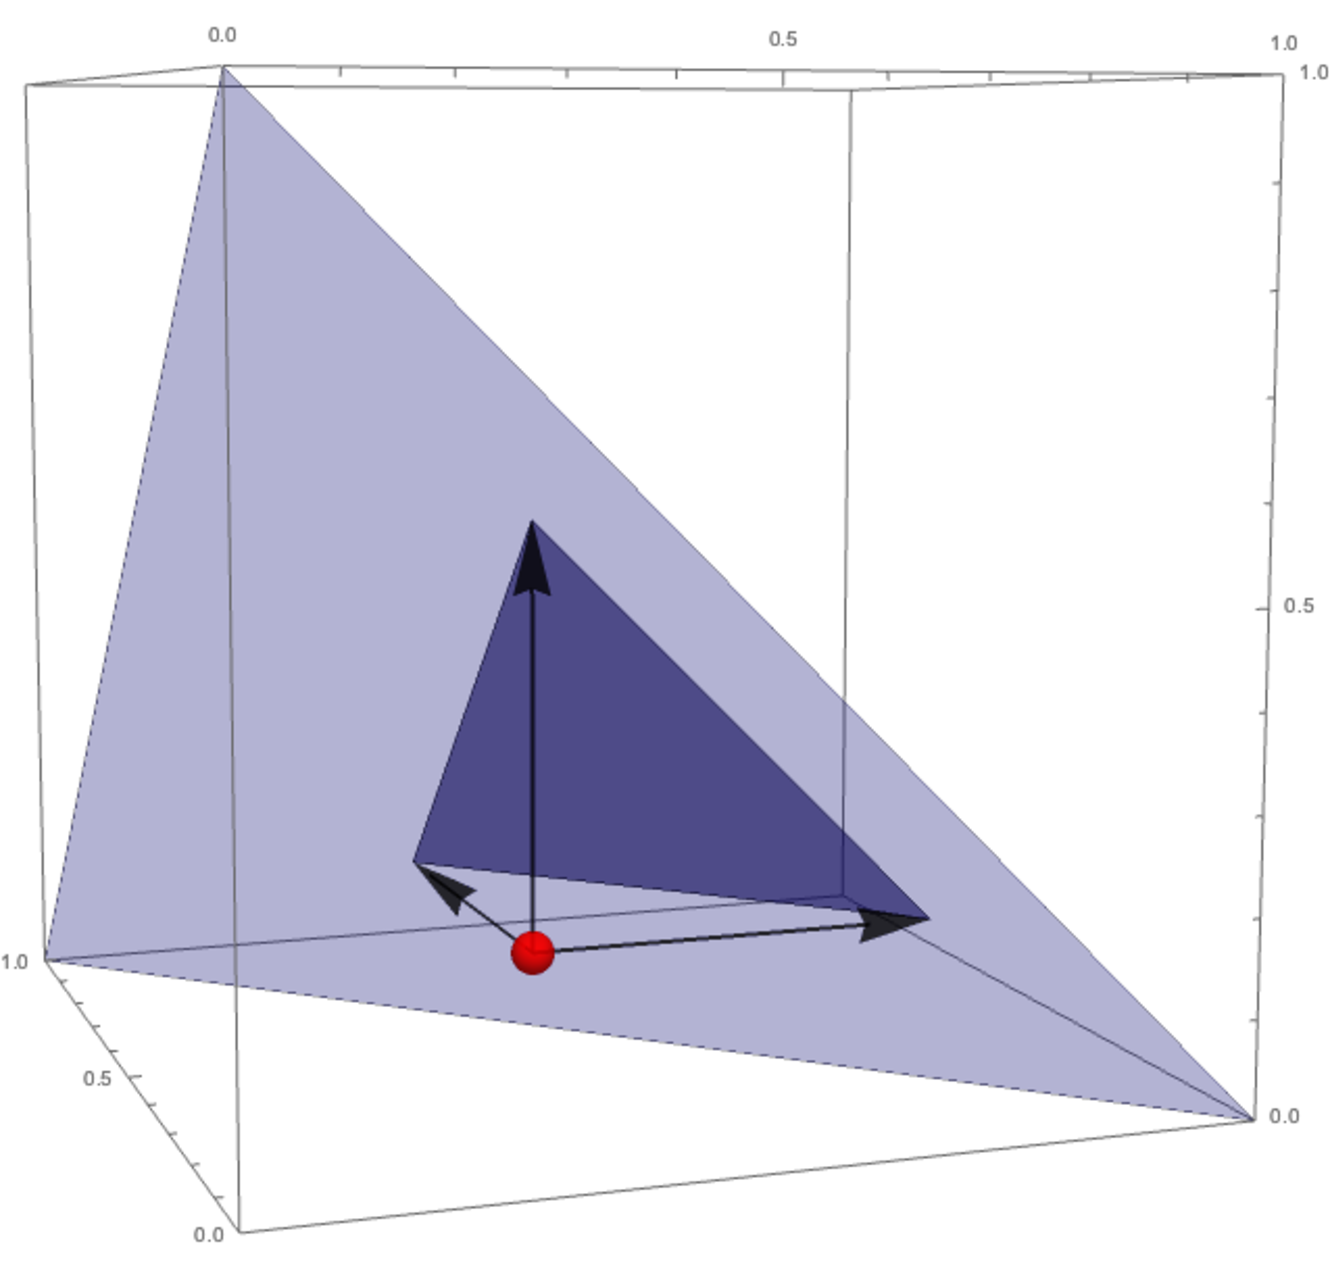
\includegraphics[width=9cm]{graphs/a_on_simplex.pdf}
\caption{ある点 $ x $ に対する $ A_x = \Set{x' \in c \Delta_n | x' \geq x} $}
\label{fig:a_on_simplex}
\end{center}
\end{figure}

さらに,$ A_x $ について以下のことが言える.

\begin{proposition} \label{prop:a_x_is_simplex}
$ \sum_{i = 1}^{n} x_i \leq c $ であるような $ x \in \mathbb{R}_+^n $ についての $ A_x = \Set{x' \in c \Delta_n | x' \geq x} $ は単体である.

\begin{proof}
\begin{align*}
A_x = & \; \Set{x' \in c \Delta_n | x' \geq x} \\
= & \; \Set{x' \in \mathbb{R}_+^n | \sum_{i = 1}^{n} x'_i = c, \; x' \geq x}
\end{align*}
あらたに変数 $ y \in \mathbb{R}_+^n $ を用意し $ y = x' - x $ とすると,
$$ A_x = \Set{y \in \mathbb{R}_+^n | \sum_{i = 1}^{n} y_i = c - \sum_{i = 1}^{n} x_i} $$
$ c' = c - \sum_{i = 1}^{n} x_i $ とすると,
$$ A_x = \Set{y \in c' \Delta_n} $$
よって $ A_x $ は単体である.
\end{proof}

\end{proposition}

ここで $ \hat{f} $ の定義を見てみると,利用しているものは $ f $ の $ A_x $ における下界値,$ c \Delta_n $ における上界値のみである.命題 \ref{prop:a_x_is_simplex} より,$ A_x, c \Delta_n $ は単体であるから,関数の単体上における下界値と上界値を調べるだけで $ \hat{f} $ の生成ができるということである.\par
次に $ \hat{f} $ が単調増加関数であることを示す.

\begin{proposition}
$ \hat{f} : \mathbb{R}_+^n \to \mathbb{R} $ は単調増加関数である.

\begin{proof}
$ \hat{f} $ の定義をするときに利用した場合分けと同じ場合分けを $ x, y $ それぞれに対して行って考える.つまり,4つに場合分けして考える.\\
(i) $ \; \sum_{i = 1}^{n} x_i \leq c, \sum_{i = 1}^{n} y_i \leq c $ である場合
\begin{align*}
x \leq y \; \Rightarrow & \; \Set{x' \in c \Delta_n | x' \geq x} \supseteq \Set{x' \in c \Delta_n | x' \geq y} \\
\Rightarrow & \; A_x \supseteq A_y \\
\Rightarrow & \; \underline{f}_{A_x} \leq \underline{f}_{A_y} \\
\Rightarrow & \; \hat{f}(x) \leq \hat{f}(y)
\end{align*}
\\
(ii) $ \; \sum_{i = 1}^{n} x_i > c, \sum_{i = 1}^{n} y_i > c $ である場合
\begin{align*}
\hat{f}(x) = \hat{f}(y) = \overline{f}_{c \Delta_n}
\end{align*}
$ \;\;\;\; $ よって $ x \leq y \Rightarrow \hat{f}(x) \geq \hat{f}(y) $ が成り立つ.\\
\\
(iii) $ \; \sum_{i = 1}^{n} x_i \leq c, \sum_{i = 1}^{n} y_i > c $ である場合
\begin{align*}
A_x \subseteq c \Delta_n \; \Rightarrow & \; \underline{f}_{A_x} \leq \overline{f}_{A_x} \leq \overline{f}_{c \Delta_n} \\
\Rightarrow & \; \underline{f}_{A_x} \leq \overline{f}_{c \Delta_n} \\
\Rightarrow & \; \hat{f}(x) \leq \hat{f}(y)
\end{align*}
\\
(iv) $ \; \sum_{i = 1}^{n} x_i > c, \sum_{i = 1}^{n} y_i \leq c $ である場合
\begin{align*}
x \leq y \; \Rightarrow & \; x_i \leq y_i \; (i = 1, ..., n) \\
\Rightarrow & \; \sum_{i = 1}^{n} x_i \leq \sum_{i = 1}^{n} y_i
\end{align*}
$ \;\;\;\; $ よって $ x \leq y $ のとき $ \sum_{i = 1}^{n} x_i > c, \sum_{i = 1}^{n} y_i \leq c $ であるような状態は存在しない.\\
\\
よって,すべての場合で以下が示された.
$$ \forall x, y \in \mathbb{R}_+^n, \; x \leq y \Rightarrow \hat{f}(x) \leq \hat{f}(y) $$
つまり,$ \hat{f} : \mathbb{R}_+^n \to \mathbb{R} $ が単調増加関数であること示された.
\end{proof}
\end{proposition}

単体上の任意の関数 $ f $ を単調増加関数 $ \hat{f} $ に変換することができたが,単体上を見てみると $ \forall x \in c \Delta_n, \; f(x) = \hat{f}(x) $ とできることが $ \hat{f} $ の定義からわかる.よって,変換後の関数を単体上で最適化することで,元の問題の単体上における最適化ができる.つまり,単調関数の単体上における最適化問題は,任意の関数の単体上における最適化問題を部分問題に含む.ただし変換の過程で,単体における関数の下界値と上界値を求めているため,それらの導出が簡単に行えるような関数に対してのみ,効率的にこの変換手法を適用することができる.\par
さらに,Rubinov ら \cite{rubinov} により,リプシッツ関数のリプシッツ定数を利用して,単体上のリプシッツ最適化問題が単調関数最適化問題に変換できることが証明されており,単調関数最適化問題はリプシッツ最適化問題を部分問題に含むことがわかる.リプシッツ最適化問題は Pint$\acute{\mbox{e}}$r \cite{pinter} により分枝限定法で解く方法が提案されているが,このような問題を部分問題に含むということである.\par
また,リプシッツ定数が未知であるリプシッツ関数の単体上における最適化問題を解く手法として,Jones ら \cite{direct} による手法である DIRECT を拡張した DISIMPL \cite{disimpl} という手法が存在する.この問題はリプシッツ定数が未知であるため,Rubinov らによる変換は利用できないが,DISIMPL では実行可能領域における下界値を算出しているため,上で示した変換手法を効率的に利用でき,このような問題も本問題の部分問題に含むだろう.\par
以上のように,本問題は多くの問題を部分問題に含み,問題が困難であることと一般性を持つことがわかった.

\section{単調関数の単体上における下界} \label{sec:lower_bound_of_monotonic_function_on_simplex}

単調関数の単体上における最適化問題の困難さについて論じてきたが,単調関数の単体以外の領域の情報を利用し,単体上の関数値の下界を得ることができる.

\begin{theorem}\label{thm:lower_bound_of_monotonic_function}
以下のような成分を持つ $ \underline{x}_A \in \mathbb{R}^n_{+} $ は,単体の任意の部分領域 $ A \subseteq c \Delta_n $ における,単調増加関数 $ f :  \mathbb{R}^n_{+} \to \mathbb{R} $ の関数値の下界 $ f(\underline{x}_A) $ を与える.
$$ \left( \underline{x}_A \right)_i = \inf_{x \in A } x_i \; , \; i = 1, ..., n $$

\begin{proof}
$ \underline{x}_A $ の定義より,$ A $ 中の任意の要素 $ x $ について $ \underline{x}_A \leq x $ が成り立つ.\\
また,$ f $ は単調増加関数であったから,$ \forall x, y \in \mathbb{R}^n_{+}, x \leq y \Rightarrow f(x) \leq f(y) $ が成り立ち,
$$ \forall x \in A, f(\underline{x}_A) \leq f(x) $$
以上により,$ f(\underline{x}_A) $ は単体の任意の部分領域 $ A $ における単調増加関数 $ f $ の下界となる.
\end{proof}

\end{theorem}

$ \underline{x}_A $ を算出するためには単体の部分領域 $ A $ における,次元ごとの最小成分を求める必要がある.$ A $ の形状がわからない場合,この処理は一般の最適化問題を解くことであるから困難である.ただし,特に $ A $ が単体である場合はその単体のすべての頂点を調べ上げるだけで $ \underline{x}_A $ の算出は完了する.なぜなら単体は凸であるから,ある次元の最小の変数値は必ず頂点が持つ.よって,$ A $ が $ n - 1 $ 次元単体であった場合,$ n $ 個の頂点を調べるだけで $ \underline{x}_A $ の算出は完了し,その計算量は $ O(n) $ である. \par
図 \ref{fig:lower_bound_of_simplex} に例を示した.$ (0.7, 0.3, 0)^T, (0, 1, 0)^T, (0, 0.3, 0.7)^T $ を頂点に持つような2次元単体 $ A $ は $ \Delta_3 $ の部分領域であるが,この単体における $ \underline{x}_{A} $ は,それぞれの次元の最小成分を集めた $ (0, 0.3, 0) $ である.図は,薄い青色の領域が $ \Delta_3 $,濃い青色の領域が $ A $,赤い点が $ \underline{x}_{A} $ を表している.\par

\begin{figure}
\begin{center}
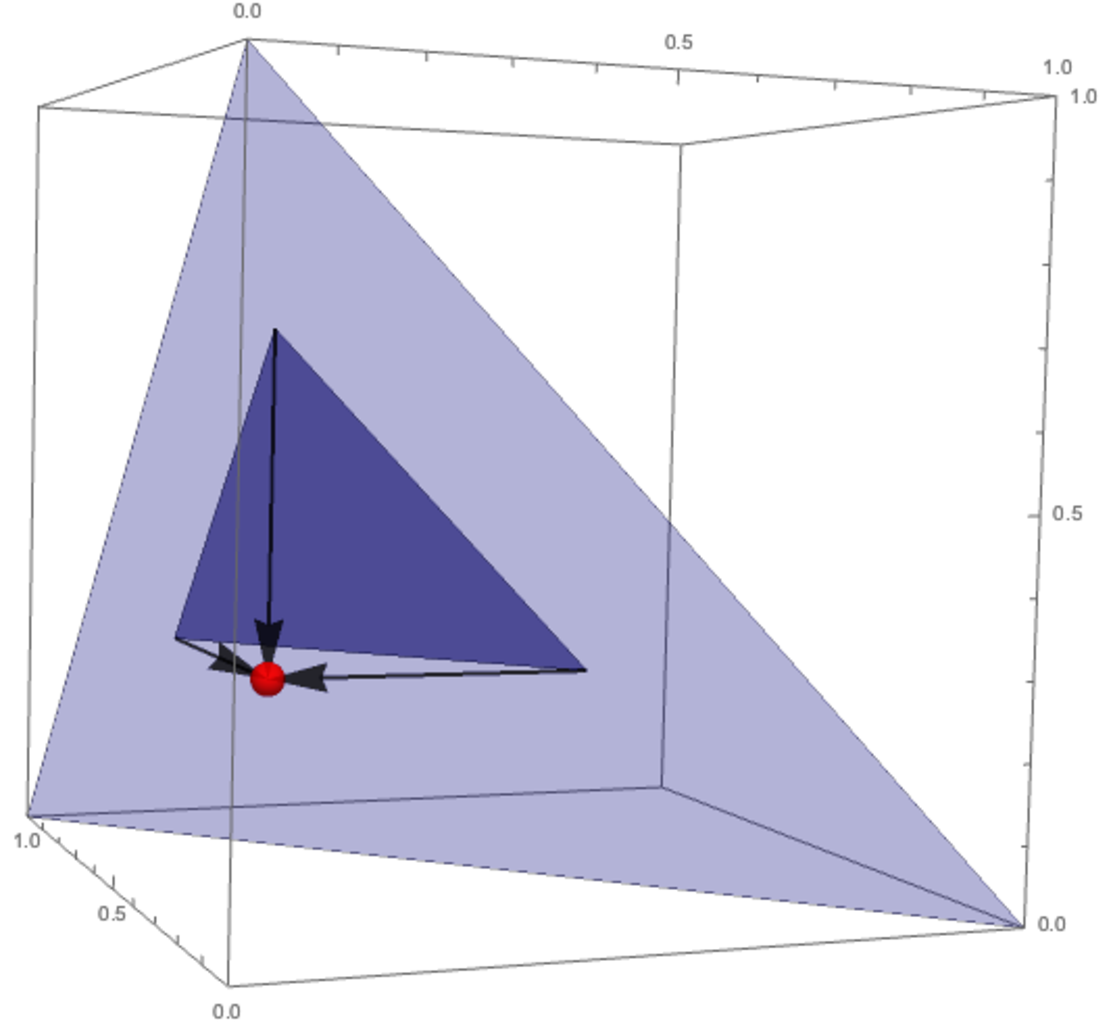
\includegraphics[width=9cm]{graphs/lower_bound_of_simplex.pdf}
\caption{$ (0.7, 0.3, 0)^T, (0, 1, 0)^T, (0, 0.3, 0.7)^T $ を頂点に持つような単体の下界を与える点}
\label{fig:lower_bound_of_simplex}
\end{center}
\end{figure}

\chapter{関連研究}

本研究で構築するアルゴリズムの中で利用する先行研究を説明する.グリッド化した単体上で分枝限定法を実行するために,まずは単体のグリッド化の定義と性質の説明を行い,次に一般的な分枝限定法のアルゴリズムの説明を行う.最後に,分枝限定法における分枝操作を行うための単体の分割方法について説明する.

\section{グリッド化した単体上における最適化} \label{sec:gridize_simplex}
Bomze, de Klerk \cite{bomze} により行なわれた,グリッド化した単体上での最適化について説明する.単体のグリッド化とは,単体上に格子を考え,格子上の点だけを抽出することである.このようなグリッド化した単体上の点の中で最も良い点を探し,それを近似解として出力する.まずは単体のグリッド化の定義を行い,グリッド数の多項式性と,近似精度について説明する.\par

\subsection{単体のグリッド化}

単体のグリッド化の定義を行う.$ m \in \mathbb{Z}_+ $ を利用して,単位単体の各辺を $ m $ 分割して得られるグリッド化された単体は以下のように表せる.
$$ \Set{ x \in \Delta_n | mx \in \mathbb{Z}_+^n } $$
次に,$ c \in \mathbb{Z}_+ $ を利用して,各辺の長さが $ c $ であるような単体 $ c \Delta_n $ をグリッド化したもの $ G(c, n, m) $ を以下のように定義する.

\begin{definition}
$$ G(c, n, m) \triangleq \Set{x \in c \Delta_n | mx \in \mathbb{Z}_+^n} $$
\end{definition}

ここで,$ c = 1 $ としたとき,$ G(1, n, m) $ は $ n - 1 $ 次元の単位単体の各辺を $ m $ 等分してグリッド化したものと同じであることがわかる.\par
さらに,単体をグリッド化したときのグリッドの総数について,以下が成り立つことがわかっている.

\begin{theorem} \label{thm:n_grid}
グリッド化された単体 $ G(c, n, m) $ が持つ点の数は二項係数を利用した以下の数となる.
$$ | G(c, n, m) | = \binom{n + mc - 1}{mc} $$
\end{theorem}

これは $ m $ を固定した場合の $ n $ の多項式であり,グリッド化した単体上を全探索しても $ n $ の多項式オーダーでアルゴリズムが完了することがわかる.\par
図 \ref{fig:grid_simplex} は $ c=1, n=4, m=2 $ としてグリッド化した単体の図である.単位単体 $ \Delta_4 $ とグリッド $ G(1, 4, 2) $ を描画している.グリッドを数えると10個であることがわかり,これは $ \binom{4 + 2 - 1}{2} $ と一致することが確認できる.\par

\begin{figure}
\begin{center}
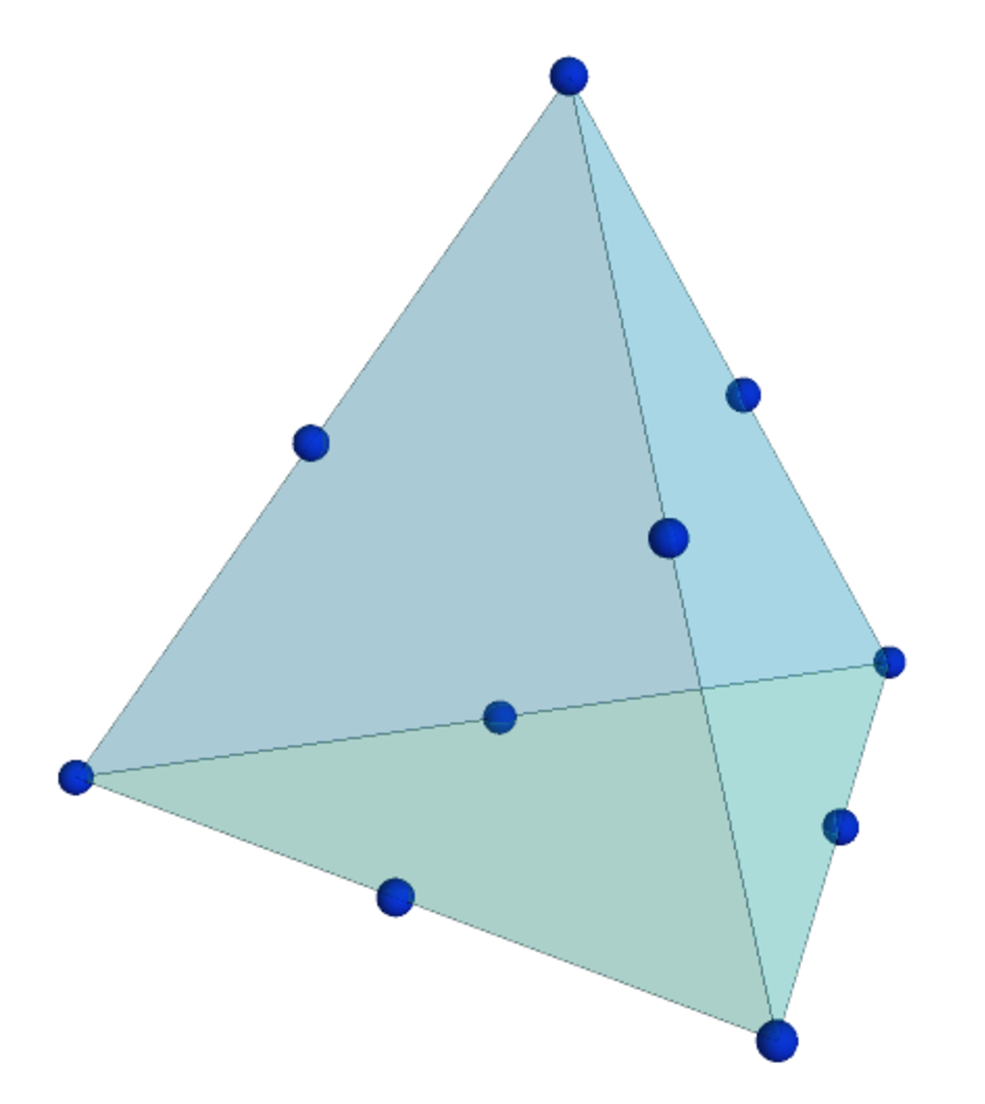
\includegraphics[width=9cm]{graphs/grid_simplex.pdf}
\caption{グリッド化された単体 $ G(1, 4, 2) $}
\label{fig:grid_simplex}
\end{center}
\end{figure}

グリッド化した単体上の点を全探索したときに多項式時間で探索が完了できることがわかったが,$ n, m $ を大きくした場合の $ \binom{n + mc - 1}{mc} $ はとても大きい数である.例えば $ c = 1, n = 10, m = 100 $ の場合,生成される点の数はおよそ $ 8.5 \times 10^{12} $ であり,多項式時間近似スキームとはいえ,全探索は難しいと容易に想像できる.よって,本研究では全探索よりも効率的な探索方法を提案し,グリッド化した単体上の最適化問題を効率的に解きたい.\par

\subsection{解の精度保証} \label{sec:rate_accuracy}

目的関数が二次多項式である場合の解の精度の保証が \cite{bomze} で以下のように与えられている.

\begin{theorem} \label{thm:quad_approximation}
目的関数を任意の二次多項式 $ f $ として,$ m \geq 2 $ であるとき,単体のグリッド化によって緩和した問題の最適解と,元の問題の最適解の間に以下の関係が成り立つ.
$$ \min_{x \in G(1, n, m)} f(x) - \min_{x \in \Delta_n} f(x) \leq \frac{1}{m} \left( \max_{x \in \Delta_n} f(x) - \min_{x \in \Delta_n} f(x) \right) $$
\end{theorem}

これは,問題の定義域の大きさに対する緩和の精度を表しており,最適化分野で一般的に利用される緩和の表現方法の一つである.定理 \ref{thm:quad_approximation} は緩和問題の最適解と元の問題の最適解の差が,問題の定義域の大きさの $ 1 / m $ 倍で抑えられることを言っている.\par
グリッド化した単体のグリッド数が多項式であることを示す定理 \ref{thm:n_grid} と,グリッド化した単体上の最適解の精度を示す定理 \ref{thm:quad_approximation} から,単体上の二次多項式最適化問題は PTAS (Polynomial Time Approximation Scheme) であることがわかった.\par
さらに研究が進み,この後に de Klerk \cite{deklerk_poly} により,目的関数が二次に限らず,多項式である場合の解の精度の保証が以下のように与えられた.\par

\begin{theorem} \label{thm:poly_approximation}
任意の $ d $ 次の多項式に対し,$ m \geq d $ であるとき,単体のグリッド化によって緩和した問題の最適解と,元の問題の最適解の間に以下の関係が成り立つ.
\begin{align*}
& \min_{x \in G(1, n, m)} f(x) - \min_{x \in \Delta_n} f(x) \leq \left( 1 - \frac{r^{\underline{d}}}{r^d} \right) \binom{2d - 1}{d} d^d \left( \max_{x \in \Delta_n} f(x) - \min_{x \in \Delta_n} f(x) \right) \\
& r^{\underline{d}} = r (r - 1) \cdots (r - d + 1)
\end{align*}
\end{theorem}

これにより,緩和問題の最適解と元の問題の最適解の差が,問題の定義域の大きさの $ \left( 1 - \frac{r^{\underline{d}}}{r^d} \right) \binom{2d - 1}{d} d^d $ 倍で抑えられることがわかった.この結果は,単体上の任意の多項式最適化問題が PTAS であることを示している.さらに,de Klerk らは単体上の多項式最適化問題が PTAS であることの別の証明を \cite{deklerk_alternative} で与えている.\par
以上のように,目的関数が多項式である場合に解の精度の保証ができることが示されており,本研究で扱う問題の,単体上の単調関数の最適化問題についても,目的関数が多項式である場合は多項式の次数を利用した解の精度の保証ができることわかった.\par

\section{分枝限定法} \label{sec:bnb}

ここでは一般的な分枝限定法について説明する.分枝限定法とは,大域的最適化の汎用アルゴリズムであり,広く利用されている.実行可能領域を分割し,それぞれの分割された領域の下界値と暫定最適値を比較することで最適解が存在し得ない領域を削除し,探索する領域を絞り込む.この操作を繰り返して効率的に探索する最適化手法である.\par
最小化問題を解く場合を考えながらアルゴリズムの説明を行う.分枝限定法は大きく分けて分枝・限定の2種類の操作から成る.分枝操作では,実行可能領域の集合からある領域 $ S $ を選択し,$ S_i \cup S_j = \phi \: (i \neq j) $ を満たす部分領域に分割する.分割の方法や分割数はアルゴリズムによって異なり,問題に適した方法で分割することが重要である.次に限定操作では,それぞれの部分領域の下界値を求める.その下界値が暫定最適値よりも大きい場合はその部分領域に最適解が存在し得ないため,その領域の探索を打ち切る.ある領域の探索を打ち切り,削除することを刈り込みと呼ぶ.領域の刈り込みを効率的に行うには,よい下界を得ること,探索中に素早くよい暫定最適値を見つけることが重要である.以上の操作をすべての領域を刈り込むまで繰り返し実行し,終了時点の最適値を問題の最適値として出力する.\par

\section{グリッド化した単体の分割} \label{sec:partition}

本節では,単体の分割方法について説明する.分枝限定法の分枝操作では実行可能領域をいくつかの部分領域に分割するが,本問題の実行可能領域は単体であるから,単体を分割する方法を考える.さらに,分枝操作は繰り返し行われるため,分割された部分領域も同様にすべて単体となっている必要がある.\par

\subsection{分割の手順}

外崎ら \cite{tonosaki} による単体の分割手法は,グリッド化された単体を,1次元少ない部分単体と,1列少ない部分単体の2つに分割する方法である.\par
まずは本研究で扱う問題,グリッド化された単位単体上の最小化問題 $ P $ を以下のように定義する.

$$
P \;
\left| \;
\begin{aligned}
& 最小化 && f(x) \\
& 条件 && x \in G(1, n, m) \\
\end{aligned}
\right.
$$

$ mb \in \mathbb{Z}_+^n $ を満たすような非負ベクトル $ b \in \mathbb{R}^n_{+} $ を利用して $ c $ を次のように与える.
$$ c \equiv 1 - \sum_{j=1}^{n} b_j > 0 $$
このとき成分のインデックスの部分集合 $ K = \{j_1, ..., j_k\} \subset \{1, ..., n\} $ を選択すると,問題 $ P $ の部分問題を以下のように定義することができる.\par

$$
P(K, b) \;
\left| \;
\begin{aligned}
& 最小化 && f(x) \\
& 条件 && \sum_{j = 1}^n x_j = 1 \\
& && mb_j \leq mx_j \in \mathbb{Z}, && j \in K \\
& && x_j = b_j, && j \not \in K
\end{aligned}
\right.
$$

$ K $ に選択されなかった成分は $ b $ の値に固定された問題となる.$ K $ に選択された成分のみを取り出した変数 $ y $ を考えると $ y \in G(c, k, m) $ となり,$ P(K, b) $ は以下の問題と等価である.\par

$$
\left| \;
\begin{aligned}
& 最小化 && f(x) \\
& 条件 && y \in G(c, k, m) \notag \\
& && y_i = x_{j_i} - b_{j_i}, && j = 1, ..., k \notag \\
& && x_j = b_j, && j \not \in K \notag
\end{aligned}
\right.
$$

この問題は各辺の大きさが $ c $ である,グリッド化された $ k - 1 $ 次元単体上の問題である.次に,$ K $ から一つのインデックス $ j_k $ を選択し $ P(K, b) $ を二つの部分問題に分割する.\par

$$
P(K, b + e_{j_k} / m) \;
\left| \;
\begin{aligned}
& 最小化 && f(x) \\
& 条件 && \sum_{j = 1}^n x_j = 1 \\
& && mb_j \leq mx_j \in \mathbb{Z}, && j \in K \backslash \{ j_k \} \\
& && mb_{j_k} + 1 \leq mx_{j_k} \in \mathbb{Z} \\
& && x_j = b_j, && j \not \in K
\end{aligned}
\right.
$$

$$
P(K \backslash \{ j_k \}, b) \;
\left| \;
\begin{aligned}
& 最小化 && f(x) \\
& 条件 && \sum_{j = 1}^n x_j = 1 \\
& && mb_j \leq mx_j \in \mathbb{Z}, && j \in K \backslash \{ j_k \} \\
& && x_j = b_j, && j \not \in K \\
& && x_{j_k} = b_{j_k}
\end{aligned}
\right.
$$

同様に,新しい単体上の変数 $ y $ を利用すると,それぞれ以下のように書き直すことができる.\par

$$
\left| \;
\begin{aligned}
& 最小化 && f(x) \\
& 条件 && y \in G(c - 1/m, k, m) \notag \\
& && y_i = x_{j_i} - b_{j_i}, && i = 1, ..., k-1 \notag \\
& && y_k = x_{j_k} - b_{j_k} - 1 / m \notag \\
& && x_j = b_j, && j \not \in K \notag
\end{aligned}
\right.
$$

$$
\left| \;
\begin{aligned}
& 最小化 && f(x) \\
& 条件 && y \in G(c, k - 1, m) \notag \\
& && y_i = x_{j_i} - b_{j_i}, && i = 1, ..., k-1 \notag \\
& && x_j = b_j, && j \not \in K \notag \\
& && x_{j_k} = b_{j_k} \notag
\end{aligned}
\right.
$$

$ P(K, b + e_{j_k} / m) $ は $ P(K, b) $ からグリッドが一列減った問題であり,$ P(K \backslash \{ j_k \}, b) $ は次元が1次元減った問題である.以上のようにグリッド化された単体を,一列減った単体と一次元減った単体に分割することができた.もともと単体には一列という概念は存在しないが,グリッド化をしたことによってこのような操作が可能になった.\par
図 \ref{fig:divided_simplices} はグリッド化した単体 $ G(1, 4, 2) $ を本手法で分割した図である.濃い青色の点の集合は一列減ったグリッド $ G(1/2, 4, 2) $ を表し,底面の水色の点の集合が一次元減ったグリッド $ G(1, 3, 2) $ を表している.元の単体は3次元単体であったが,底面の水色の単体は2次元単体,つまり平面上の正三角形となっており,一次元減っていることがわかる.また,青色の点の集合を見てみると,こちらは次元に変化はなく,変わらず3次元単体であるが,グリッドが一列削られていることがわかる.

\begin{figure}
\begin{center}
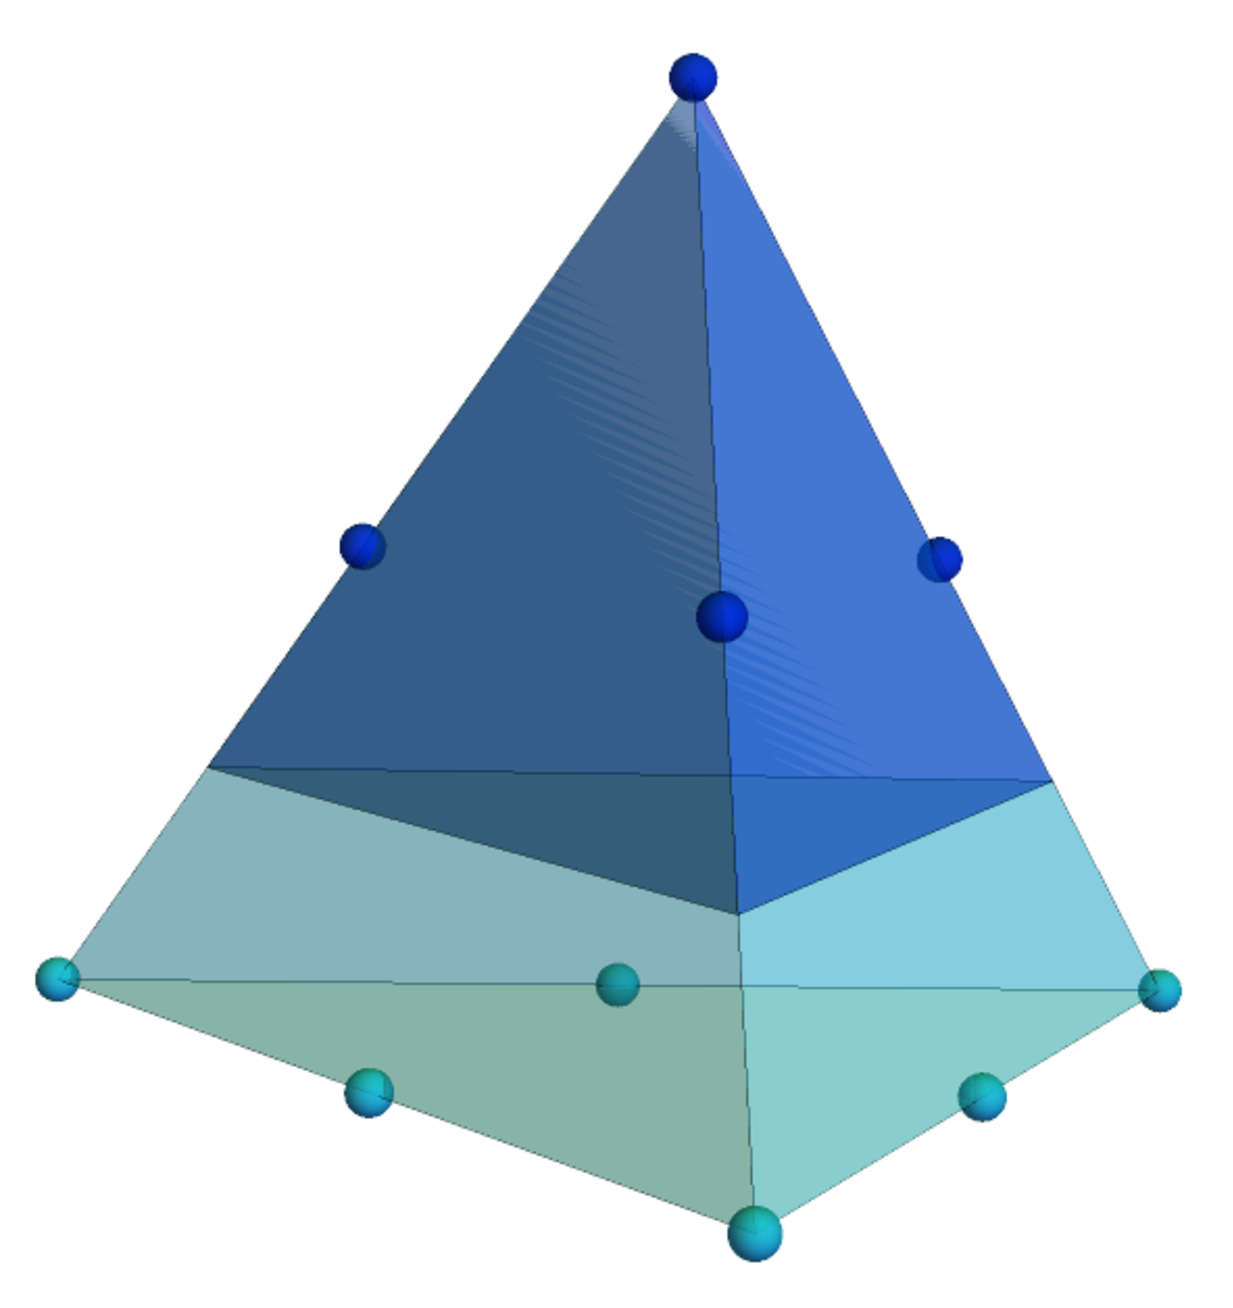
\includegraphics[width=9cm]{graphs/divided_simplices.pdf}
\caption{2つに分割されたグリッド化された単体}
\label{fig:divided_simplices}
\end{center}
\end{figure}

\subsection{部分問題のグリッド数}

定理 \ref{thm:n_grid} より,分割された問題 $ P(K, b + e_{j_k} / m), P(K \backslash \{ j_k \}, b) $ の定義域のグリッド数は以下になることがわかる.
$$ | G(c - 1/m, k, m) | = \binom{k + mc - 2}{mc - 1} $$
$$ | G(c, k - 1, m) | = \binom{k + mc - 2}{mc} $$
また,二項係数の性質として以下が知られている.
$$ \binom{k + mc - 1}{mc} = \binom{k + mc - 2}{mc - 1} + \binom{k + mc - 2}{mc} $$
ゆえに,以下のように元の単体のグリッド数は部分問題のグリッド数の和になることが確認できる.
$$ | G(c, k, m) | = | G(c - 1/m, k, m) | + | G(c, k - 1, m) | $$
以上のことから,この分枝操作を繰り返すとすべての部分問題の実行可能領域はただ一点のみを含む単体になり,その総数は $ \binom{k + mc - 1}{mc} $ である.\par

\subsection{分割数の性質} \label{sec:number_of_partition}

分枝限定法において問題は繰り返し部分問題に分割されるが,問題をノードに持つ木構造を考えることができる.分割される前の問題を親ノードとして,分割された部分問題を子ノードとすると,アルゴリズムが進行するにつれて木は子ノードを増やして大きくなる.本章で説明した分割によって生成される木を $ T $ とすると,問題は2分割されるため $ T $ は2分木である.さらに,問題を完全に分割し切った場合,部分問題の実行可能領域はただ一点を持つ単体となるが,この部分問題は $ T $ の末端の葉ノードにあたる.そして $ G(1, n, m) $ を根ノードとする二分木 $ T $ のノード数について以下のことが言える.

\begin{theorem} \label{thm:total_node}
$ T $ の総ノード数は $ 2 \binom{n + m - 1}{m} - 1 $ である
\end{theorem}
\begin{proof}
数学的帰納法で示す.$ r = \binom{n + m - 1}{m} $ とおくと,$ r $ は $ T $ の葉の数を表す.$ q < r $ であるような $ q $ に対して,$ q $ を葉ノードの総数とする二分木の総ノード数は $ 2q - 1 $ であると仮定する.\\
次に $ T $ の根ノードを親に持つような二つの部分木を $ T_1, T_2 $ とし,それらの葉ノードの数を $ r_1, r_2 $ とすると,$ r = r_1 + r_2 $ が成り立つ.さらに,$ r_1, r_2 \leq r - 1 $ であるから仮定より,$ T_1, T_2 $ の総ノード数は $ 2r_1 - 1, 2r_2 - 1 $ である.\\
よって,$ T $ の総ノード数は
$$ (2r_1 - 1) + (2r_2 - 1) + 1 = 2(r_1 + r_2) - 1 = 2r - 1 $$
\end{proof}

定理 \ref{thm:total_node} により,$ G(1, n, m) $ を根ノードとして分枝限定法を実行したとき,分割回数が $ 2 \binom{n + m - 1}{m} - 1 $ ,つまり $ n $ の多項式であることが示された.

\chapter{グリッド化した単体上の分枝限定法}

本章では,グリッド化した単体上の単調関数を分枝限定法で最適化する提案手法の説明をする.分枝限定法において,領域の分割方法,下界の良さはアルゴリズムの速度に対してとても重要であることを \ref{sec:bnb} 節で述べたが,本研究では単調関数の下界に定理  \ref{thm:lower_bound_of_monotonic_function} で得られるものを利用し,分割方法は \ref{sec:partition} 節で説明したもの利用する.\par

\section{分割する次元の選択}

% TODO: わかりやすく
分枝限定法において,分割された部分問題が良い関数値を持つことは,その部分領域が良い下界を持つことにつながり,その下界によってその領域を削除しやすくなる.さらに同時に,良い暫定解を得ることにもつながるため,部分問題が良い関数値を持つことはアルゴリズムの早い収束に対して重要である.本節では,部分領域が良い関数値を持つような \ref{sec:partition} 節における成分のインデックス $ j_k $ の選び方,つまり,問題を分割する次元の決定方法について論じる.\par
\ref{sec:partition} 節の問題 $ P(K, b) $ では,元の変数 $ x $ の代わりに $ y \in G(c, k, m) $ となるような変数 $ y $ が取り直されている.$ G(c, k, m) $ は成分のインデックス $ j_k $ を選択することで二つの部分領域 $ G(c, k-1, m), \; G(c-1/m, k, m) $ に分割される.選択された $ j_k $ 成分について詳しく見てみると,$ G(c, k - 1, m) $ では $ j_k $ 成分の値 $ x_{j_k} $ は $ b_{j_k} $ に固定されており,これに対応する $ y \in G(c, k, m) $ における変数値 $ y_k $ は最小値 $ 0 $ となる.\par
本問題で扱っている関数は単調増加関数であるから,ある成分のインデックス $ k $ に着目したとき,$ y_k $ が大きくなれば関数値は単調に増加し,逆に $ y_k $ が小さくなれば関数値は単調に減少する.よって,関数値に対して大きなインパクトを与えている成分のインデックス $ k $ を探し出し,$ k $ 成分について単体を分割すると,部分問題 $ P(K \backslash \{ k \}, b) $ の $ k $ 成分の変数値は最小値に固定され,関数値は小さくなると予想できる.\par
次に,そのような大きなインパクトを与えている成分のインデックス $ k $ の探し方を考える.$ G(c, k, m) $ の頂点の集合を考えると,それらは $ c $ 倍した $ k $ 次の単位行列 $ I $ の列を取り出したものとなっている.つまり,$ k $ 個の頂点の成分は以下のようになっている.
$$ (c, 0, 0, ..., 0)^T, (0, c, 0, ..., 0)^T, (0, 0, c, ..., 0)^T, ..., (0, 0, 0, ..., c)^T $$
ある $ i $ 成分に着目すると,$ i $ 番目の頂点の $ i $ 成分の値は $ c $ で,それ以外の頂点の $ i $ 成分の値は $ 0 $ である.ここで,全ての頂点について関数値を調べ,最も悪い関数値を持った頂点を $ j $ 番目の頂点であるとする.さらに,関数の単調性を考えてみると,頂点の $ j $ 成分の値のインパクトが大きいために関数値が悪くなっているのではないかと予想できる.そこで,よい関数値を持った部分領域を切り出すために,$ j $ について単体を分割し,部分問題の $ j $ 成分の変数値を最小値に固定する.\par
分割元の単体を入力として受け取り,本手法によって分割する次元を決定するプログラムの疑似コードを Algorithm \ref{algo:cutting_dimension} に示した.\par

\begin{algorithm}
\caption{Decide the cutting dimension of a simplex}
\label{algo:cutting_dimension}
\begin{algorithmic}[1]
\Function{DecideCuttingDimension}{simplex}
\State Initialize $ worst\_value $
\State Initialize $ dimension $
\For{each $ vertex $ of $ simplex $}
\State $ function\_value := \Call{ObjectiveFunctionValue}{vertex} $
\If{$ function\_value \geq worst\_value $}
\State $ worst\_value := function\_value $
\State $ dimension := \Call{GetDimension}{vertex} $
\EndIf
\EndFor
\State \Return $ dimension $
\EndFunction
\end{algorithmic}
\end{algorithm}

\section{部分問題の保持}

本節では分枝限定法の分枝操作によって分割された部分問題の,プログラム上での扱い方について説明する.\ref{sec:number_of_partition} 節で述べた通り,問題の分割は木構造を持つ.アルゴリズムは問題 $ P $ を根ノードとして始まり,アルゴリズムが進行するにつれて木のノード数は指数的に増大する.分枝限定法ではすべての葉ノードの問題を分割する必要があるが,大きなサイズの問題を解く場合,コンピュータのメモリ上に全ての葉ノードのオブジェクトを保持し続けることは困難となる.この問題を解決するために,すべての葉ノードを保持するのでなく,分割の情報を表現する二分木 $ T $ を保持し,葉ノードが表す部分問題はそのつど二分木の情報から生成する.\par

\subsection{二分木の構成}

プログラム中における二分木の作り方を説明する.二分木のノードは部分問題を表現し,問題を分割した際に単体を分割した次元をノードに保存する.$ P(K, b) $ を分割すると二つの部分問題が生成されるが,グリッドが一列減った部分問題 $ P(K, b + e_{j_k} / m) $ は左の子ノードに,一次元減った部分問題 $ P(K \backslash \{ j_k \}, b) $ は右の子ノードに挿入する.以上のルールに従って二分木を構成することで,二分木に保持された情報から,ある葉ノードが表す問題における単体の形状を復元することができる.\par
$ n = 3, m = 3 $ の問題を解いた際の二分木 $ T $ の構造の例を図 \ref{fig:simplex_tree} に示した.アルゴリズムの開始状態は $ K = \{1, 2, 3\} \; , \; b = (0, 0, 0)^T $ である.緑色の丸に囲まれた数字は単体を分割した次元を表し,グリッドが一列減った問題は下側の子ノード,次元が減った問題は上側の子ノードとして書いた.ここで,実際にプログラムが保持するのは図における緑色の部分のみ,つまり単体を分割した次元と二分木の構造のみであり,問題や単体のオブジェクトは保持しない.どのようにこの二分木からノードが表す問題を生成するかを次で説明する.\par

\begin{figure}
\begin{center}
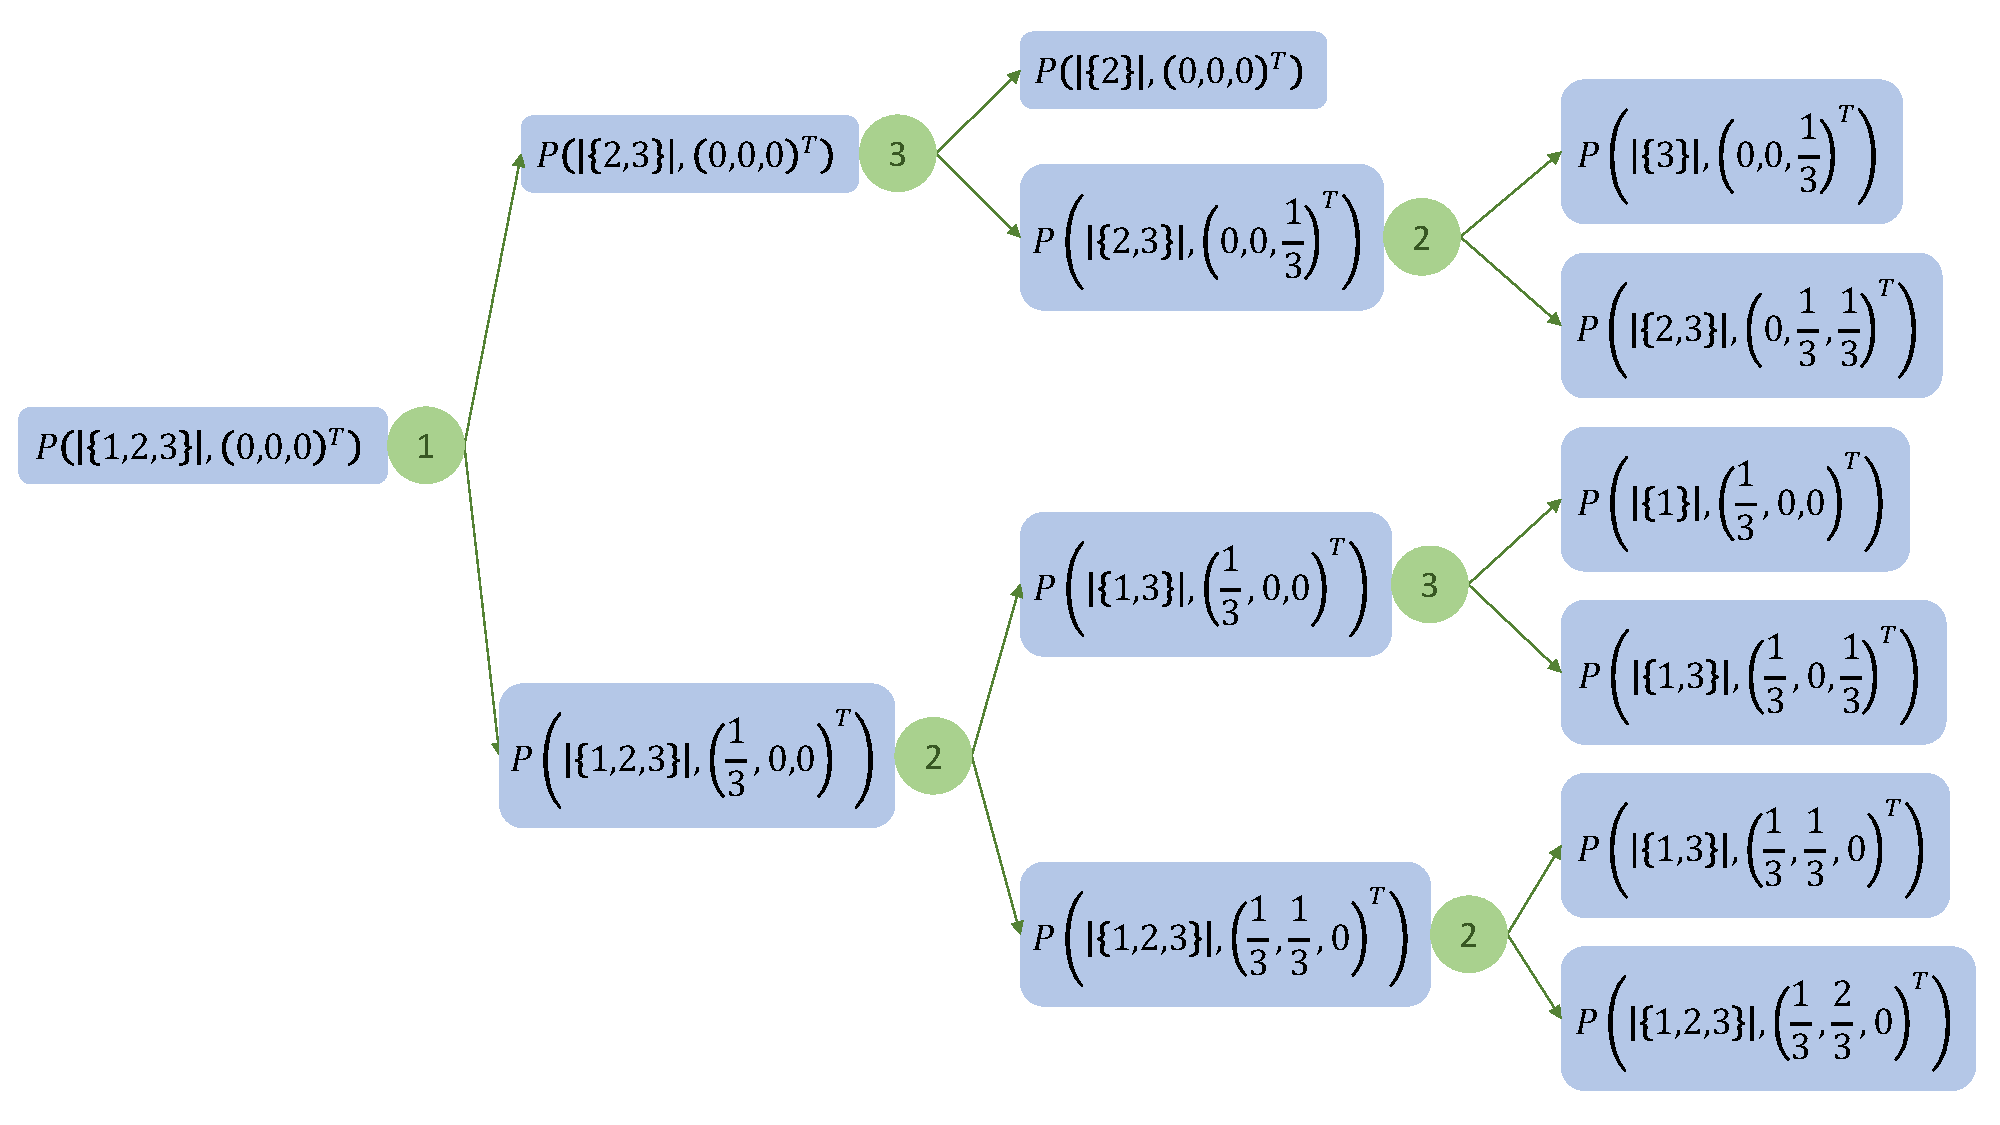
\includegraphics[width=17cm]{graphs/simplex_tree.pdf}
\caption{$ n = 3, m = 3 $ の問題を解いたときの二分木 $ T $ の例}
\label{fig:simplex_tree}
\end{center}
\end{figure}

\subsection{二分木から問題を生成する方法} \label{sec:generate_problem_from_btree}

二分木の情報から,葉ノードが表す問題の実行可能領域である単体を生成する方法を示す.調べたい葉ノードから根ノードまで,親ノードをたどる.その際,左右どちらの子ノードであるかの情報と分割された次元を取得し,その二つの情報から葉ノードが表す部分問題を一意に再現できる.ある葉ノードを入力とし,そのノードが表現する部分問題の実行可能領域単体を返す疑似コードを Algorithm \ref{algo:regenerate_simplex_from_btree} に示した.この処理の計算量は,ノードが最も深い場所にある場合に最悪となるが,木の深さは高々 $ n + m $ であるから,最悪計算量は $ O(n + m) $ である.\par

\begin{algorithm}
\caption{Regenerate the simplex from the binary tree}
\label{algo:regenerate_simplex_from_btree}
\begin{algorithmic}[1]
\Function{RegenerateSimplex}{$ node $}
\State $ simplex := \Call{GenerateUnitSimplex} $
\While{$ parent := \Call{parent}{node} $}
\State $ cutting\_dimension := binary\_tree[parent] $
\If{$ node $ is left node}
\State $ simplex := \Call{CutOneRow}{simplex, cutting\_dimension} $
\ElsIf{$ node $ is right node}
\State $ simplex := \Call{CutOneDimension}{simplex,  cutting\_dimension} $
\EndIf
\State $ node := parent $
\EndWhile
\State \Return $ simplex $
\EndFunction
\end{algorithmic}
\end{algorithm}

\section{低次元の単体の処理}

アルゴリズムが進行するにつれ,分割された問題の次元は小さくなる.ここで分割の情報を保持する二分木 $ T $ を考えてみると,木の末端に近い部分には低次元の問題しか存在せず,木の末端に近いということはそれらの数がとても多いことが容易に想像できる.よって,低次元の問題を効率良く処理することはアルゴリズムの速度に対して重要である.\par
外崎ら \cite{tonosaki} による研究では単体が点になるまで分割を行っていた.例えば1次元単体 (線分) を分割するとき,その単体は一次元減った単体 (点) と一点が取り除かれた単体 (線分) に分割される.下界によって刈り込まれる場合を除き,この処理を単体の分割数回 ($ m $ 回) 繰り返すことによってやっと全ての単体が点となりアルゴリズムが終了する.分割を繰り返すことでアルゴリズムのオーバーヘッドはかさむため,低次元の問題は別の単純なアルゴリズムで探索し,速度を向上したい.低次元の問題一つ一つにおける実行時間の改善は小さいものであるが,その数はとても多いため,アルゴリズム全体として速度の大幅な改善が期待される.\par
分割が進み,問題が2次元,つまり実行可能領域が線分になった場合は単純に全てのグリッドの関数値を評価する.この処理は,単体が $ m $ 分割されている場合は $ O(m) $ の処理となる.疑似コードを Algorithm \ref{algo:line_search} に示した.\par

\begin{algorithm}
\caption{Line search}
\label{algo:line_search}
\begin{algorithmic}[1]
\Function{LineSearch}{$ line $}
\For{each $ point $ of $ line $}
\State $ function\_value := \Call{ObjectiveFunctionValue}{point} $
\If{$ function\_value < current\_optima $}
\State $current\_optima := function\_value $
\EndIf
\EndFor
\EndFunction
\end{algorithmic}
\end{algorithm}

\section{アルゴリズム}

これまでに説明した処理をまとめた疑似コードを Algorithm \ref{algo:main} に示した.これは単調増加関数をグリッド化された単体上で最小化するアルゴリズムである.\par
ここで,多くの最適化手法ではアルゴリズムにパラメータが存在し,またその数が多い場合もあり,パラメータを決定するのが困難であることがある.しかし,本アルゴリズムにおけるパラメータは $ m $ のみであり,さらにこの $ m $ は求めたい解の精度から決定することができることが \ref{sec:rate_accuracy} 節によってわかっている.よって,本アルゴリズムはパラメータフリーなアルゴリズムであると言えるだろう.\par

\begin{algorithm}
\caption{Optimize monotonic function on a simplex}
\label{algo:main}
\begin{algorithmic}[1]
\State Initialize $ binary\_tree $
\State Initialize $ current\_optima $
\State $ i $ := 0
\While{$ true $}
\State $ nodes := i $ th row of $ binary\_tree $
\If{$ nodes $ are empty}
\Break
\EndIf
\For{each $ node $ of $ nodes $}
\State $ simplex = \Call{RegenerateSimplex}{node} $
\State $ lower\_bound := \Call{CalculateLowerBound}{simplex} $
\If{$ current\_optima \leq lower\_bound $}
\Continue
\EndIf
\If{$ simplex $ is a line}
\State $ \Call{LineSearch}{simplex} $
\Continue
\EndIf
\If{$ current\_optima \geq $ any vertices of $ simplex $}
\State Replace $ current\_optima $
\EndIf
\State $ cutting\_dimension = \Call{DecideCuttingDimension}{simplex} $
\State $ binary\_tree[node] := cutting\_dimension $
\EndFor
\EndWhile
\State \Return $ current\_optima $
\end{algorithmic}
\end{algorithm}

\section{並列化} \label{sec:parallel}

本アルゴリズムの並列化について述べる.分割の情報を保持する二分木 $ T $ における,同一列のノードには相互に依存性はないため,少なくとも列ごとに処理が完了していることを保証すればアルゴリズムを並列化できる.Algorithm \ref{algo:cutting_dimension} による分割する次元の計算や,Algorithm \ref{algo:line_search} による線形探索を並行して実行できるため,アルゴリズム全体に対して速度の向上が図れるかもしれない.\par
ただし,$ G(1, n, m) $ を実行可能領域とする問題に対して,Algorithm \ref{algo:cutting_dimension} のオーダーは高々 $ O(n) $ で,Algorithm \ref{algo:line_search} は高々 $ O(m) $ であるため,それほど重い処理ではない.よって問題の大きさによっては,大きな速度の改善が見られない,もしくはスレッドの切り替えのオーバーヘッドがかさみむしろ改悪することも考えうる.\par
具体的には,Algorithm \ref{algo:main} における 10 - 23 行目を並列化できる.

\section{計算量の解析} \label{sec:analysis}

Algorithm \ref{algo:main} の計算量を考える.本アルゴリズムは4行目から始まる while ループがメインループである.まずはその内部で利用している主な処理を解析する.10行目で二分木から単体を生成している処理は \ref{sec:generate_problem_from_btree} 節で説明した通り高々 $ O(n + m) $,11行目で下界を与える点を計算する処理は \ref{sec:lower_bound_of_monotonic_function_on_simplex} 節の通り $ O(n) $,16行目の線形探索は Algorithm \ref{algo:line_search} を利用して高々 $ O(m) $,最後に,22行目の分割する次元を決定する処理は Algorithm \ref{algo:cutting_dimension} により単体の頂点を調べ上げれば完了するため $ O(n) $ である.以上により,$ m $ を固定したときのすべてのサブモジュールの計算量は高々 $ O(n) $ であることがわかった.\par
さらに,メインループの繰り返し回数について考えてみると,最悪の場合,つまり下界による刈り込みが一切できない場合に,分割の情報を保持する二分木 $ T $ の最大ノード数回繰り返される.定理 \ref{thm:total_node} により,$ T $ の最大ノード数は $ 2 \binom{n + m - 1}{m} - 1 $ であることがわかっており,これが最悪計算量となる.$ 2 \binom{n + m - 1}{m} - 1 $ は $ n $ に対する多項式であるが,多項式の多項式は多項式である性質から,Algorithm \ref{algo:main} 全体の計算量は $ n $ の多項式である.\par
\ref{sec:gridize_simplex} 節で説明した de Klerk による単体のグリッド化では,グリッドの総数は $ \binom{n + m - 1}{m} $ であり,グリッドを全探索することで多項式時間で探索が完了するとしていた.分枝限定法を利用した本アルゴリズムの計算量も多項式時間であるが,最悪計算量はそれよりも大きい.ただし,単体上の単調関数の下界を利用した刈り込み操作による効率化が期待できる.本アルゴリズムの有用性を確認するために次章で実験結果を説明する.

\chapter{実験}

\ref{sec:gridize_simplex} 節で説明した de Klerk による手法と,提案する手法であるグリッド化した単体を分枝限定法で最適化する手法の性能を,実験によって比較する.\ref{sec:analysis} 節で計算量の解析をした通り,最悪計算量は提案手法の方が悪いが,提案手法は下界値を利用した刈り込み操作が行えるため,効率的に刈り込みができれば既存手法よりも良い結果を出すことが期待できる.\par
また,それぞれのアルゴリズムはグリッド化した単体上における大域的最適化アルゴリズムであるから,単体のグリッド上における最適解を必ず得ることができ,\ref{sec:rate_accuracy} 節の通り解の精度保証がされているため,精度についての実験はここでは不要である.\par

\section{実験の条件}

本実験では,単体上の単調増加関数の最小化問題を解いて両アルゴリズムを比較するが,単体上の単調関数最適化問題はこれまであまり研究されておらず,ベンチマーク問題が少ない.そこで,Bagirov, Rubinov \cite{bagirov} による単体上における IPH 関数最適化の研究で利用されているベンチマーク問題を利用する.IPH 関数とは,Increasing positively homogeneous function のことであり,単調増加性を有しており,本問題のベンチマーク問題としても利用できる.\par
本手法では単体のグリッド化を行うが,事前にグリッドの分割数を決める必要がある.\ref{sec:rate_accuracy} 節で解の精度について説明した通り,グリッド化した単体上の解の精度はグリッド数によって決まるため,実用する場合は,必要な精度によって問題のグリッド数を決定するべきである.しかし,ここでは性能を比較することが目的であるため,$ m = 100 $ として全ての実験を行う.\par
また,\ref{sec:parallel} 節でアルゴリズムの並列化について説明した通り,提案手法は並列化することができたが,既存手法は並列化できていない.平等に実験を行うため,提案手法は並列化したものとそうでないものの両方を計測し,アルゴリズム自体の比較は並列化していないもの同士で行う.\par
実験は Intel Core i7-4790K 4.00GHz, 8 Processors を持つ計算機で行い,プログラムは C++ で記述した.\par

\section{問題}

$ f_1 $ は以下のような maxmin 関数の特殊ケースである.\par

\begin{align*}
& f_1(x) = \max_{i \in I} \{a_i x_i \} + \min_{j \in I} \{b_j x_j \} \\
& a_i = 2 + 0.5 i, \;\; i \in I \\
& b_j = (j + 2) (n - j + 2), \;\; j \in I \\
& I = \Set{1, 2, ..., n}
\end{align*}

$ f_2 $ は以下のような内積の計算を含む関数である.ここで,$ x, y $ の内積は $ \langle x, y \rangle = \sum_{i = 1}^{n} x_i y_i $ と表すとする.\par

\begin{align*}
& f_2(x) = \max_{i = 1, ..., 40} \langle a^i, x \rangle + \min_{j = 1, ..., 20} \langle b^j, x \rangle \\
& (a^i)_k = \frac{20i}{k(1 + | i - k |)}, \;\; k = 1, 2, ..., n \\
& (b^j)_k = 5 | \sin{(j)} \sin{(k)} |, \;\; k = 1, 2, ..., n
\end{align*}
\section{実験結果}

問題の次元を変化させ,それぞれのアルゴリズムの計算時間を計測した.de Klerk の手法を de Klerk,提案する手法を BnB,それを並列化したものを Parallel BnB と呼ぶこととする.\par
表 \ref{tbl:f_1_table} は目的関数を $ f_1 $ として解いた場合の各アルゴリズムの実行時間で,図 \ref{fig:f_1_time} はそのグラフである.数字が書かれていない部分は,実行時間がかかりすぎたため計測しなかった.de Klerk と BnB を比較してみると,BnB は4次元以上の問題で de Klerk よりも実行時間が短い.特に6次元について見てみると,BnB は de Klerk のおよそ 12\% の時間で最適化が完了しており,提案手法が効率的に動いていることがわかる.また,BnB と Parallel BnB を比較してみると,6次元,7次元では計算時間がおよそ 65\% になっており,並列化による高速化ができていることが確認できる.\par
次に,$ f_2 $ についての結果を確認する.表 \ref{tbl:f_2_table} は目的関数を $ f_2 $ とした場合の実行時間で,図 \ref{fig:f_2_time} はそのグラフである.関数 $ f_2 $ はベクトルの内積計算を行っているため,$ f_1 $ よりも関数値を求めるのに時間がかかり,すべての場合で $ f_1 $ よりも時間がかかっている.ただし,この場合でも $ f_1 $ の場合と同様に,4次元以上の問題で de Klerk よりも BnB が計算時間が短い.さらに BnB と Parallel BnB を比べることで並列化について見てみると,4次元,5次元の場合は並列化によって計算時間が約 38\% になっており,これは $ f_1 $ の場合よりも効率がよい.\par
%この理由は,$ f_2 $ は関数値を求めるのに時間がかかるため,1スレッドの計算時間は長くなり,そのことによって並列化の効率が $ f_1 $ の場合よりも良くなっていることだと考えられる.\par
次に,BnB, Parallel BnB において,単調関数の単体上における下界値を利用して刈り込まれたノードの数を,問題と次元ごとに比較する.ここでノードの数とは,\ref{sec:partition} 節における,単体を保持する二分木 $ T $ のノードの数であり,その最大数は定理 \ref{thm:total_node} によって $ 2 \binom{n + m - 1}{m} - 1 $ であることがわかっている.いま,$ m = 100 $ として実験を行っているため,ノードの最大数は $ 2 \binom{n + 99}{100} - 1 $ である.目的関数が $ f_1 $ の場合の刈り込まれたノードの数を表 \ref{tbl:f_1_eliminated},図 \ref{fig:f_1_eliminated} に,$ f_2 $ の場合を表 \ref{tbl:f_2_eliminated},図 \ref{fig:f_2_eliminated} に示した.どちらの関数についても,次元が増えると刈り込まれるノードの数が増えていることがわかる.特に $ f_1 $ では6次元以上の場合で 90\% 以上のノードが刈り込まれており,とても効率よく分枝限定法が動いていることがわかる.このために,$ f_1 $ の実験において BnB が de Klerk に対してより実行時間が短かったと考えられる.\par
% TODO: より深い考察

\newpage

\begin{table}[h]
\caption{$ f_1 $ の各アルゴリズムの実行時間 (秒)}
\label{tbl:f_1_table}
\begin{center}
\begin{tabular}{|c|r|r|r|} \hline
次元 & de Klerk & BnB & Parallel BnB \\ \hline
2 & 0.00014 & 0.00048 & 0.00049 \\
3 & 0.0064 & 0.011 & 0.017 \\
4 & 0.19 & 0.063 & 0.048 \\
5 & 4.96 & 0.98 & 0.67 \\ 
6 & 106.60 & 12.55 & 8.23 \\
7 & 1961.75 & 143.43 & 98.60 \\
8 & - & - & 952.27 \\
9 & - & - & 11885.24 \\ \hline
\end{tabular}
\end{center}
\end{table}

\begin{figure}[h]
\begin{center}
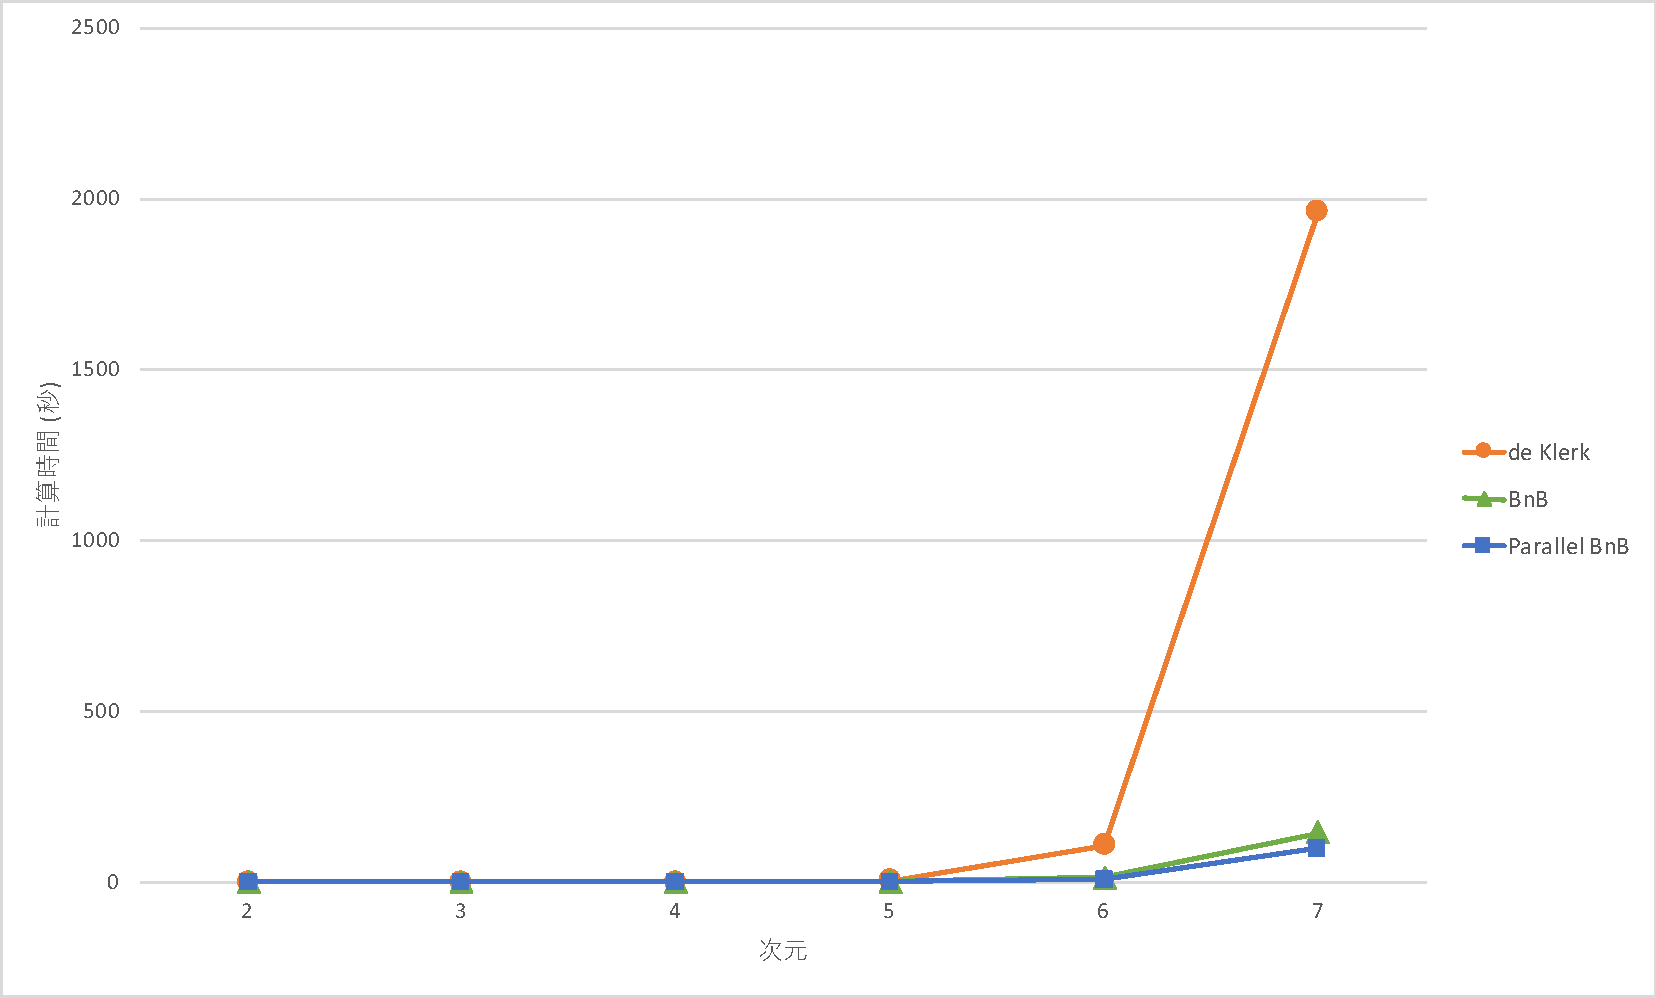
\includegraphics[width=14cm]{graphs/f_1_time.pdf}
\caption{$ f_1 $ の各アルゴリズムの実行時間}
\label{fig:f_1_time}
\end{center}
\end{figure}

\newpage

\begin{table}[h]
\caption{$ f_2 $ の各アルゴリズムの実行時間 (秒)}
\label{tbl:f_2_table}
\begin{center}
\begin{tabular}{|c|r|r|r|} \hline
次元 & de Klerk & BnB & Parallel BnB \\ \hline
2 & 0.0033 & 0.0062 & 0.0055 \\
3 & 0.23 & 0.24 & 0.20 \\
4 & 8.16 & 6.29 & 2.36 \\
5 & 276.75 & 168.24 & 65.34 \\ 
6 & - & - & 1134.25 \\
7 & - & - & 16641.55 \\ \hline
\end{tabular}
\end{center}
\end{table}

\begin{figure}[h]
\begin{center}
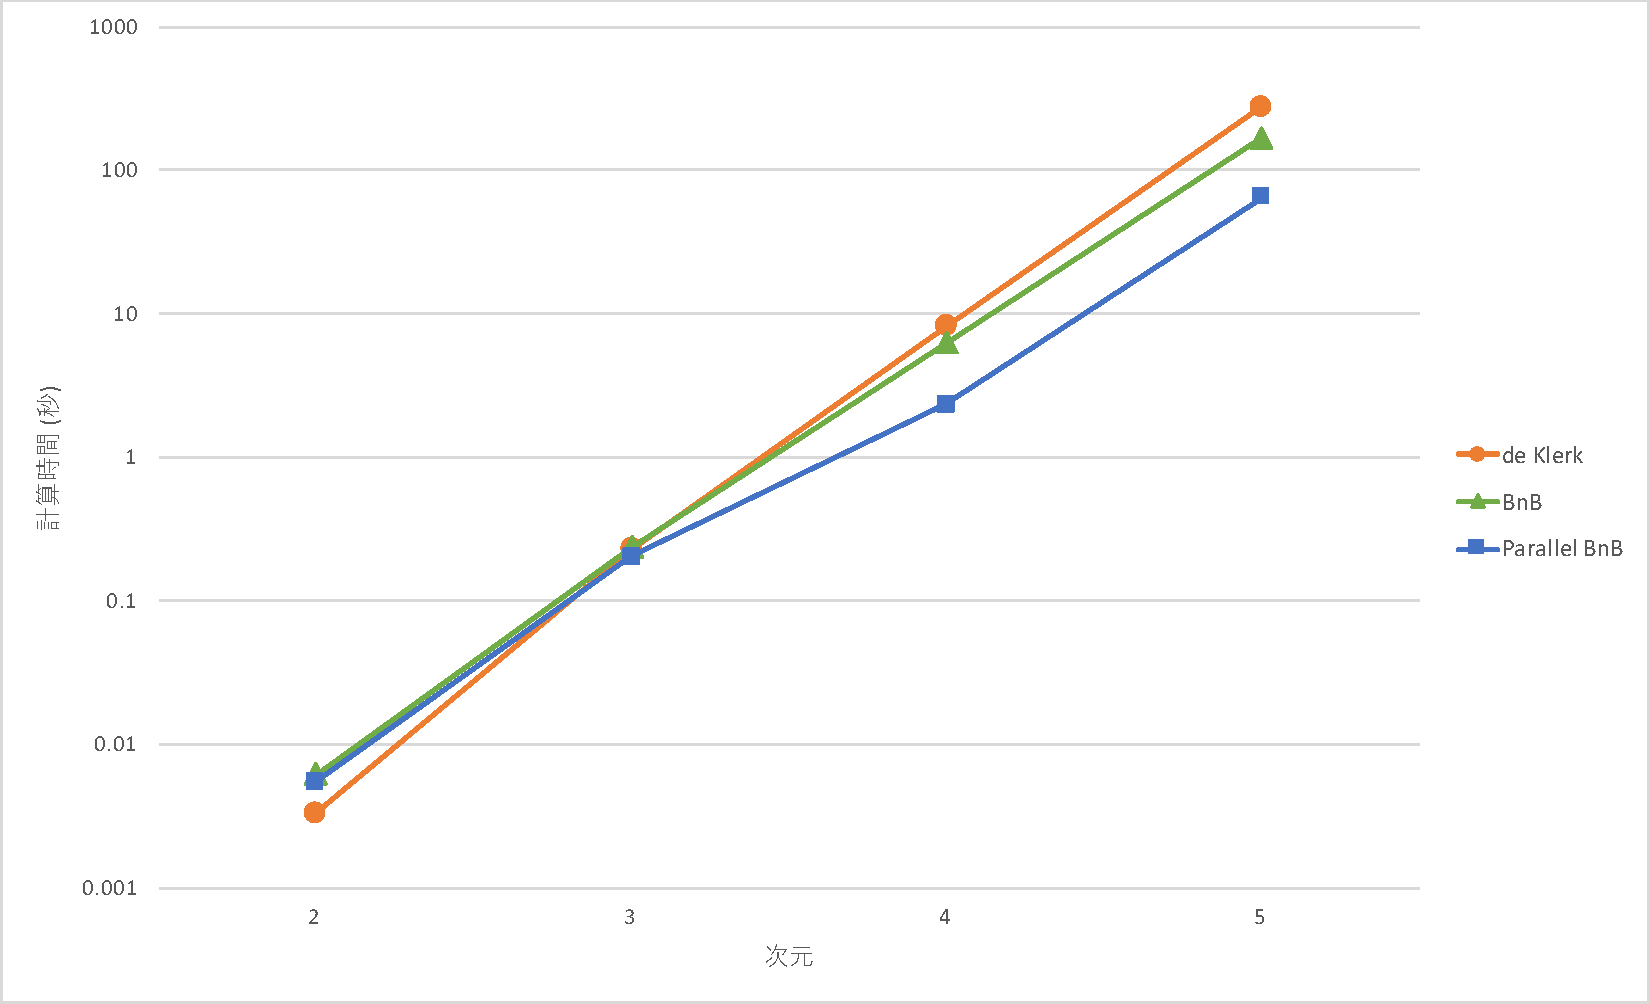
\includegraphics[width=14cm]{graphs/f_2_time.pdf}
\caption{$ f_2 $ の各アルゴリズムの実行時間}
\label{fig:f_2_time}
\end{center}
\end{figure}

\newpage

\begin{table}[h]
\caption{$ f_1 $ の下界によって刈り込まれたノードの数}
\label{tbl:f_1_eliminated}
\begin{center}
\begin{tabular}{|c|r|r|r|} \hline
次元 & 刈り込まれたノードの数 & ノードの最大数 & 刈り込まれたノードの割合 \\ \hline
2 & 0 & 201 & 0\% \\
3 & 3,781 & 10,301 & 36.71\% \\
4 & 244,326 & 353,701 & 69.08\% \\
5 & 7,739,229 & 9,196,251 & 84.16\% \\
6 & 175,321,588 & 193,121,291 & 90.78\% \\
7 & 3,221,353,517 & 3,411,809,491 & 94.42\% \\
8 & 50,348,126,591 & 52,151,945,091 & 96.54\% \\ 
9 & 688,850,091,267 & 704,051,258,741 & 97.84\% \\ \hline
\end{tabular}
\end{center}
\end{table}

\begin{figure}[h]
\begin{center}
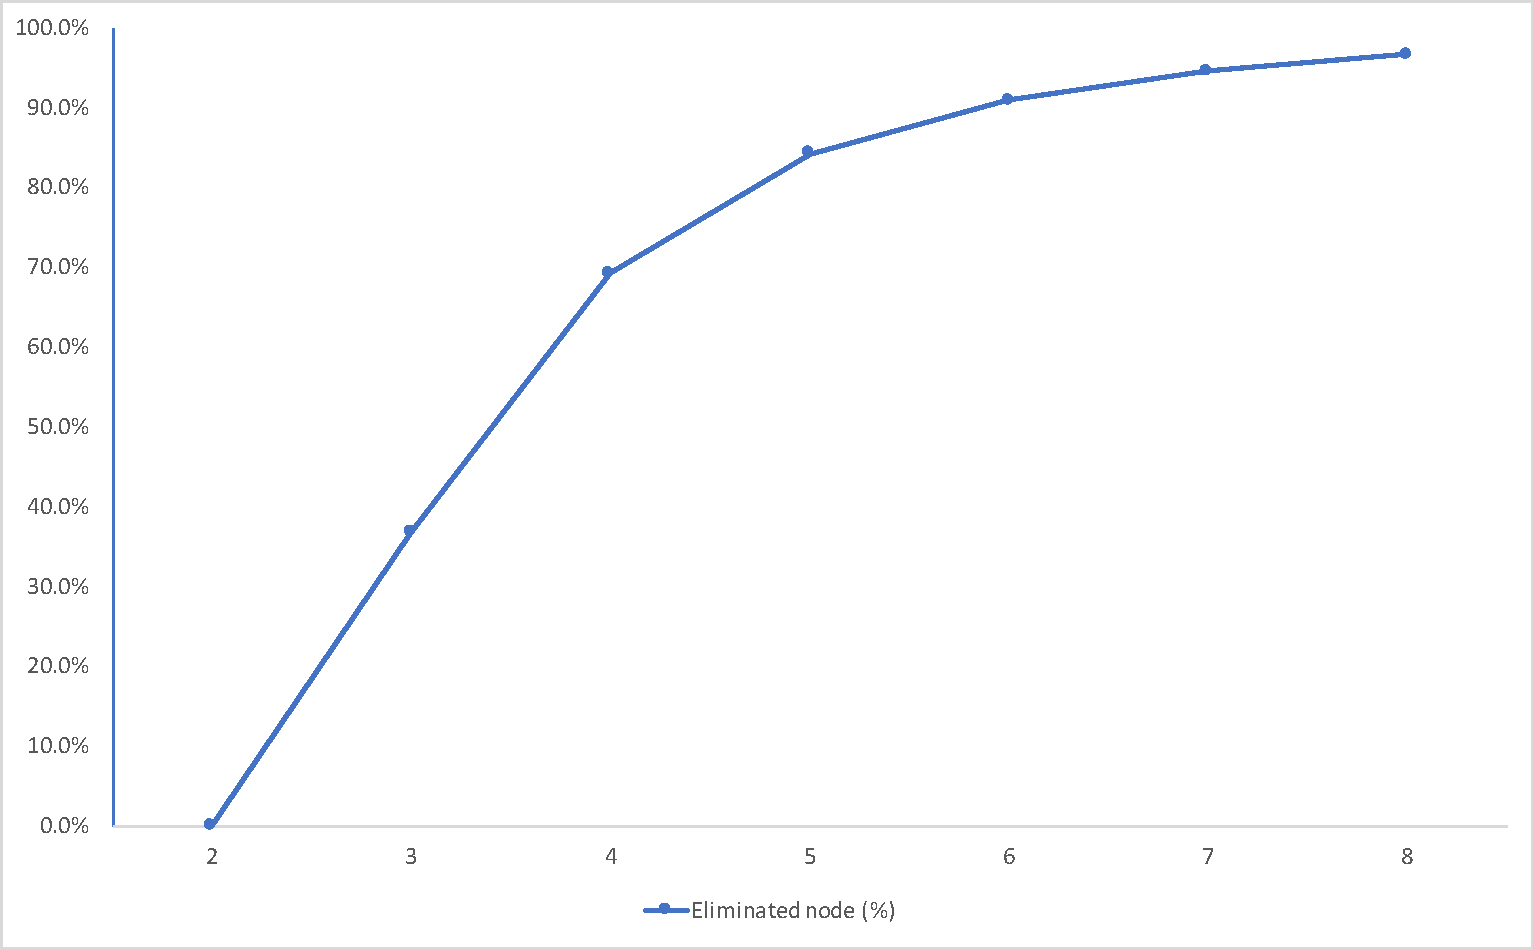
\includegraphics[width=13.5cm]{graphs/f_1_eliminated.pdf}
\caption{$ f_1 $ の下界によって刈り込まれたノードの割合}
\label{fig:f_1_eliminated}
\end{center}
\end{figure}

\newpage

\begin{table}[h]
\caption{$ f_2 $ の下界によって刈り込まれたノードの数}
\label{tbl:f_2_eliminated}
\begin{center}
\begin{tabular}{|c|r|r|r|} \hline
次元 & 刈り込まれたノードの数 & ノードの最大数 & 刈り込まれたノードの割合 \\ \hline
2 & 0 & 201 & 0\% \\
3 & 379 & 10,301 & 3.68\% \\
4 & 63,177 & 353,701 & 17.86\% \\
5 & 2,817,758 & 9,196,251 & 30.64\% \\
6 & 89,770,014 & 193,121,291 & 46.48\% \\ 
7 & 1,980,717,332 & 3,411,809,491 & 58.05\% \\ \hline
\end{tabular}
\end{center}
\end{table}

\begin{figure}[h]
\begin{center}
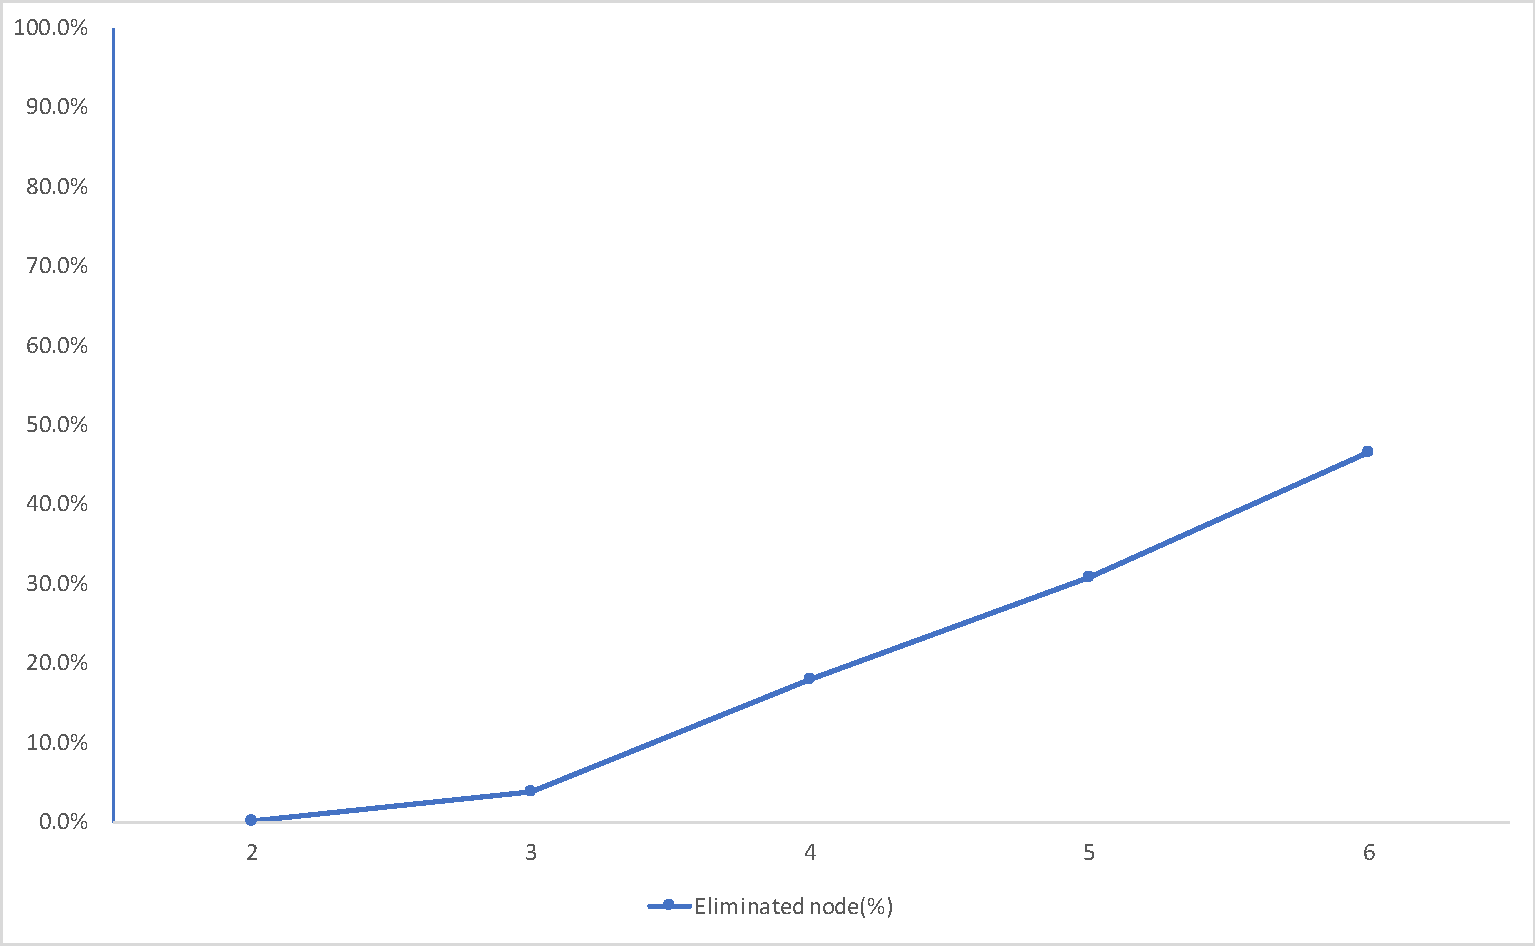
\includegraphics[width=13.5cm]{graphs/f_2_eliminated.pdf}
\caption{$ f_2 $ の下界によって刈り込まれたノードの割合}
\label{fig:f_2_eliminated}
\end{center}
\end{figure}

\chapter{結論}

本研究では単体上における単調関数の最適化を行った.本問題はこれまであまり研究されていないため,まずは問題の解析を行った.単体における下界が得られる関数を単調関数に変換することができることを示し,単体上の単調関数として最適化を行うことで,変換前の問題を解くことができることがわかった.それによって,本問題の困難さと一般性を示した.\par
単体をグリッド化して最適化を行う de Klerk の手法を利用して,グリッド化した単体上での分枝限定法を構築した.そして,本アルゴリズムが多項式時間近似スキームであることを示した.計算実験により,ほとんどの場合で本手法が既存手法よりも実行時間が短いことを示し,本手法の有用性を確かめた.\par
最後に今後の課題として,単体上における単調関数のよりよい下界を発見すること,より効率のよい分枝規則を発見することを挙げる.\par

\chapter*{謝辞}
\addcontentsline{toc}{chapter}{\numberline{}謝辞}

研究を進めるにあたり,多くの指導を頂いた久野誉人先生,佐野良夫先生に深く感謝いたします.また,様々な議論を通じて多くの知識や示唆を頂いたシステム数理研究室のみなさまに感謝します.最後に,学生生活をサポートしてくれた家族と友人たちに感謝します.

\newpage

\addcontentsline{toc}{chapter}{\numberline{}参考文献}
\renewcommand{\bibname}{参考文献}

\begin{thebibliography}{1}

\bibitem{bagirov}
A. Bagirov, and A. Rubinov,
\newblock {\it Global minimization of increasing positively homogeneous functions over the unit simplex},
\newblock Annals of Operations Research 98.1-4 (2000), pp.171-187.

\bibitem{bomze}
I. Bomze, and E. de Klerk,
\newblock {\it Solving standard quadratic optimization problems via linear, semidefinite and copositive programming},
\newblock Journal of Global Optimization 24.2 (2002), pp.163-185.

\bibitem{deklerk_survey}
E. de Klerk,
\newblock {\it The complexity of optimizing over a simplex, hypercube or sphere: a short survey},
\newblock Central European Journal of Operations Research 16.2 (2008), pp.111-125.

\bibitem{deklerk}
E. de Klerk, D. Hertog, and G. Elabwabi,
\newblock {\it On the complexity of optimization over the standard simplex},
\newblock European journal of operational research 191.3 (2008), pp.773-785.

\bibitem{deklerk_poly}
E. de Klerk, M. Laurent, and P. Parrilo,
\newblock {\it A PTAS for the minimization of polynomials of fixed degree over the simplex},
\newblock Theoretical Computer Science 361.2 (2006), pp.210-225.

\bibitem{deklerk_alternative}
E. de Klerk, M. Laurent, and Z. Sun,
\newblock {\it An alternative proof of a PTAS for fixed-degree polynomial optimization over the simplex},
\newblock Mathematical Programming 151.2 (2015), pp.433-457.

\bibitem{direct}
D. Jones, C. Perttunen, and B. Stuckman,
\newblock {\it Lipschitzian optimization without the Lipschitz constant},
\newblock Journal of Optimization Theory and Applications 79.1 (1993), pp.157-181.

\bibitem{pinter}
J. Pint$\acute{\mbox{e}}$r,
\newblock {\it Global Optimization in Action},
\newblock Kluwer Academic Publishers, Volume 6, (1996).

\bibitem{disimpl}
R. Paulavi$\breve{\mbox{c}}$ius, and J. $\breve{\mbox{Z}}$ilinskas,
\newblock {\it Simplicial Lipschitz Optimization Without Lipschitz Constant},
\newblock Simplicial Global Optimization (2014), pp.61-86.

\bibitem{rubinov}
A. Rubinov, and M. Andramonov,
\newblock {\it Lipschitz programming via increasing convex-along-rays functions},
\newblock Optimization Methods and Software 10.6 (1999), pp.763-781.

\bibitem{tuy}
H. Tuy,
\newblock {\it Monotonic optimization: Problems and solution approaches},
\newblock SIAM Journal on Optimization 11.2 (2000), pp.464-494.

\bibitem{tuy_survey}
H. Tuy, F. Al-Khayyal, and P. Thach,
\newblock {\it Monotonic optimization: Branch and cut methods},
\newblock Essays and Surveys in Global Optimization. Springer US (2005), pp.39-78.

\bibitem{tonosaki}
外崎真造,
\newblock 非凸2次制約付き配合計画問題のロバスト最適化,
\newblock 筑波大学システム情報工学研究科修士学位論文 (2010)

\end{thebibliography}

\end{document}
